\documentclass[a4paper,12pt,twoside]{memoir}

% Castellano
\usepackage[spanish,es-tabla]{babel}
\selectlanguage{spanish}
\usepackage[utf8]{inputenc}
\usepackage[T1]{fontenc}
\usepackage{lmodern} % Scalable font
\usepackage{microtype}
\usepackage{placeins}
\usepackage{tabularx}

\RequirePackage{booktabs}
\RequirePackage[table]{xcolor}
\RequirePackage{xtab}
\RequirePackage{multirow}

% Links
\PassOptionsToPackage{hyphens}{url}\usepackage[colorlinks]{hyperref}
\hypersetup{
	allcolors = {red}
}

% Ecuaciones
\usepackage{amsmath}

% Rutas de fichero / paquete
\newcommand{\ruta}[1]{{\sffamily #1}}

% Párrafos
\nonzeroparskip

% Huérfanas y viudas
\widowpenalty100000
\clubpenalty100000

% Imágenes

% Comando para insertar una imagen en un lugar concreto.
% Los parámetros son:
% 1 --> Ruta absoluta/relativa de la figura
% 2 --> Texto a pie de figura
% 3 --> Tamaño en tanto por uno relativo al ancho de página
\usepackage{graphicx}
\newcommand{\imagen}[3]{
	\begin{figure}[!h]
		\centering
		\includegraphics[width=#3\textwidth]{#1}
		\caption{#2}\label{fig:#1}
	\end{figure}
	\FloatBarrier
}

% Comando para insertar una imagen sin posición.
% Los parámetros son:
% 1 --> Ruta absoluta/relativa de la figura
% 2 --> Texto a pie de figura
% 3 --> Tamaño en tanto por uno relativo al ancho de página
\newcommand{\imagenflotante}[3]{
	\begin{figure}
		\centering
		\includegraphics[width=#3\textwidth]{#1}
		\caption{#2}\label{fig:#1}
	\end{figure}
}

% El comando \figura nos permite insertar figuras comodamente, y utilizando
% siempre el mismo formato. Los parametros son:
% 1 --> Porcentaje del ancho de página que ocupará la figura (de 0 a 1)
% 2 --> Fichero de la imagen
% 3 --> Texto a pie de imagen
% 4 --> Etiqueta (label) para referencias
% 5 --> Opciones que queramos pasarle al \includegraphics
% 6 --> Opciones de posicionamiento a pasarle a \begin{figure}
\newcommand{\figuraConPosicion}[6]{%
  \setlength{\anchoFloat}{#1\textwidth}%
  \addtolength{\anchoFloat}{-4\fboxsep}%
  \setlength{\anchoFigura}{\anchoFloat}%
  \begin{figure}[#6]
    \begin{center}%
      \Ovalbox{%
        \begin{minipage}{\anchoFloat}%
          \begin{center}%
            \includegraphics[width=\anchoFigura,#5]{#2}%
            \caption{#3}%
            \label{#4}%
          \end{center}%
        \end{minipage}
      }%
    \end{center}%
  \end{figure}%
}

%
% Comando para incluir imágenes en formato apaisado (sin marco).
\newcommand{\figuraApaisadaSinMarco}[5]{%
  \begin{figure}%
    \begin{center}%
    \includegraphics[angle=90,height=#1\textheight,#5]{#2}%
    \caption{#3}%
    \label{#4}%
    \end{center}%
  \end{figure}%
}
% Para las tablas
\newcommand{\otoprule}{\midrule [\heavyrulewidth]}
%
% Nuevo comando para tablas pequeñas (menos de una página).
\newcommand{\tablaSmall}[5]{%
 \begin{table}
  \begin{center}
   \rowcolors {2}{gray!35}{}
   \begin{tabular}{#2}
    \toprule
    #4
    \otoprule
    #5
    \bottomrule
   \end{tabular}
   \caption{#1}
   \label{tabla:#3}
  \end{center}
 \end{table}
}

%
% Nuevo comando para tablas pequeñas (menos de una página).
\newcommand{\tablaSmallSinColores}[5]{%
 \begin{table}[H]
  \begin{center}
   \begin{tabular}{#2}
    \toprule
    #4
    \otoprule
    #5
    \bottomrule
   \end{tabular}
   \caption{#1}
   \label{tabla:#3}
  \end{center}
 \end{table}
}

\newcommand{\tablaApaisadaSmall}[5]{%
\begin{landscape}
  \begin{table}
   \begin{center}
    \rowcolors {2}{gray!35}{}
    \begin{tabular}{#2}
     \toprule
     #4
     \otoprule
     #5
     \bottomrule
    \end{tabular}
    \caption{#1}
    \label{tabla:#3}
   \end{center}
  \end{table}
\end{landscape}
}

%
% Nuevo comando para tablas grandes con cabecera y filas alternas coloreadas en gris.
\newcommand{\tabla}[6]{%
  \begin{center}
    \tablefirsthead{
      \toprule
      #5
      \otoprule
    }
    \tablehead{
      \multicolumn{#3}{l}{\small\sl continúa desde la página anterior}\\
      \toprule
      #5
      \otoprule
    }
    \tabletail{
      \hline
      \multicolumn{#3}{r}{\small\sl continúa en la página siguiente}\\
    }
    \tablelasttail{
      \hline
    }
    \bottomcaption{#1}
    \rowcolors {2}{gray!35}{}
    \begin{xtabular}{#2}
      #6
      \bottomrule
    \end{xtabular}
    \label{tabla:#4}
  \end{center}
}

%
% Nuevo comando para tablas grandes con cabecera.
\newcommand{\tablaSinColores}[6]{%
  \begin{center}
    \tablefirsthead{
      \toprule
      #5
      \otoprule
    }
    \tablehead{
      \multicolumn{#3}{l}{\small\sl continúa desde la página anterior}\\
      \toprule
      #5
      \otoprule
    }
    \tabletail{
      \hline
      \multicolumn{#3}{r}{\small\sl continúa en la página siguiente}\\
    }
    \tablelasttail{
      \hline
    }
    \bottomcaption{#1}
    \begin{xtabular}{#2}
      #6
      \bottomrule
    \end{xtabular}
    \label{tabla:#4}
  \end{center}
}

%
% Nuevo comando para tablas grandes sin cabecera.
\newcommand{\tablaSinCabecera}[5]{%
  \begin{center}
    \tablefirsthead{
      \toprule
    }
    \tablehead{
      \multicolumn{#3}{l}{\small\sl continúa desde la página anterior}\\
      \hline
    }
    \tabletail{
      \hline
      \multicolumn{#3}{r}{\small\sl continúa en la página siguiente}\\
    }
    \tablelasttail{
      \hline
    }
    \bottomcaption{#1}
  \begin{xtabular}{#2}
    #5
   \bottomrule
  \end{xtabular}
  \label{tabla:#4}
  \end{center}
}



\definecolor{cgoLight}{HTML}{EEEEEE}
\definecolor{cgoExtralight}{HTML}{FFFFFF}

%
% Nuevo comando para tablas grandes sin cabecera.
\newcommand{\tablaSinCabeceraConBandas}[5]{%
  \begin{center}
    \tablefirsthead{
      \toprule
    }
    \tablehead{
      \multicolumn{#3}{l}{\small\sl continúa desde la página anterior}\\
      \hline
    }
    \tabletail{
      \hline
      \multicolumn{#3}{r}{\small\sl continúa en la página siguiente}\\
    }
    \tablelasttail{
      \hline
    }
    \bottomcaption{#1}
    \rowcolors[]{1}{cgoExtralight}{cgoLight}

  \begin{xtabular}{#2}
    #5
   \bottomrule
  \end{xtabular}
  \label{tabla:#4}
  \end{center}
}



\graphicspath{ {./img/} }

% Capítulos
\chapterstyle{bianchi}
\newcommand{\capitulo}[2]{
	\setcounter{chapter}{#1}
	\setcounter{section}{0}
	\setcounter{figure}{0}
	\setcounter{table}{0}
	\chapter*{\thechapter.\enskip #2}
	\addcontentsline{toc}{chapter}{\thechapter.\enskip #2}
	\markboth{#2}{#2}
}

% Apéndices
\renewcommand{\appendixname}{Apéndice}
\renewcommand*\cftappendixname{\appendixname}

\newcommand{\apendice}[1]{
	%\renewcommand{\thechapter}{A}
	\chapter{#1}
}

\renewcommand*\cftappendixname{\appendixname\ }

% Formato de portada
\makeatletter
\usepackage{xcolor}
\newcommand{\tutor}[1]{\def\@tutor{#1}}
\newcommand{\course}[1]{\def\@course{#1}}
\definecolor{cpardoBox}{HTML}{E6E6FF}
\def\maketitle{
  \null
  \thispagestyle{empty}
  % Cabecera ----------------
\noindent
\includegraphics[width=\textwidth]{cabecera}\vspace{1cm}%
  \vfill
  % Título proyecto y escudo informática ----------------
  \colorbox{cpardoBox}{%
    \begin{minipage}{.8\textwidth}
      \vspace{.5cm}\Large
      \begin{center}
      \textbf{TFG del Grado en Ingeniería Informática}\vspace{.6cm}\\
      \textbf{\LARGE\@title{}}
      \end{center}
      \vspace{.2cm}
    \end{minipage}

  }%
  \hfill\begin{minipage}{.20\textwidth}
    
\includegraphics[width=\textwidth]{escudoInfor}
  \end{minipage}
  \vfill
  % Datos de alumno, curso y tutores ------------------
  \begin{center}%
  {%
    \noindent\LARGE
    Presentado por \@author{}\\ 
    en Universidad de Burgos --- \@date{}\\
    Tutores: \@tutor{}\\
  }%
  \end{center}%
  \null
  \cleardoublepage
  }
\makeatother

\newcommand{\nombre}{Hugo de la Cámara Saiz} %%% cambio de comando

% Datos de portada
\title{\textbf{Estudio y configuración de un sistema ELK}}
\author{\nombre}
\tutor{Jesús Manuel Maudes Raedo y Antonio Canepa Oneto}
\date{\today}

\begin{document}

\maketitle


\newpage\null\thispagestyle{empty}\newpage


%%%%%%%%%%%%%%%%%%%%%%%%%%%%%%%%%%%%%%%%%%%%%%%%%%%%%%%%%%%%%%%%%%%%%%%%%%%%%%%%%%%%%%%%
\thispagestyle{empty}


\noindent
\includegraphics[width=\textwidth]{cabecera}\vspace{1cm}

\noindent D. Jesús Manuel Maudes Raedo, profesor del departamento de nombre departamento, área de nombre área y D. Antonio Canepa Oneto profesor del departamento de nombre departamento, área de nombre área.

\noindent Expone:

\noindent Que el alumno D. \nombre, con DNI 71566986W, ha realizado el Trabajo final de Grado en Ingeniería Informática titulado \textit{Estudio y configuración de un sistema ELK}. 

\noindent Y que dicho trabajo ha sido realizado por el alumno bajo la dirección del que suscribe, en virtud de lo cual se autoriza su presentación y defensa.

\begin{center} %\large
En Burgos, {\large \today}
\end{center}

\vfill\vfill\vfill

% Author and supervisor
\begin{minipage}{0.45\textwidth}
\begin{flushleft} %\large
Vº. Bº. del Tutor:\\[2cm]
D. Jesús Manuel Maudes Raedo
\end{flushleft}
\end{minipage}
\hfill
\begin{minipage}{0.45\textwidth}
\begin{flushleft} %\large
Vº. Bº. del co-tutor:\\[2cm]
D. Antonio Canepa Oneto
\end{flushleft}
\end{minipage}
\hfill

\vfill

% para casos con solo un tutor comentar lo anterior
% y descomentar lo siguiente
%Vº. Bº. del Tutor:\\[2cm]
%D. nombre tutor


\newpage\null\thispagestyle{empty}\newpage




\frontmatter

% Abstract en castellano
\renewcommand*\abstractname{Resumen}
\begin{abstract}
La gestión de datos y monitorización de sistemas forma parte del esqueleto básico de toda empresa del siglo XXI a la hora de potenciar y maximizar el rendimiento de la misma. 

Este trabajo de fin de grado se centrará en explorar lo que nos ofrecen los elementos de un sistema basado en las herramientas ELK (ElasticSearch, Logstash y Kibana) para monitorizar la información y gestionar los datos a la hora de tomar decisiones.

Nos vamos a enfocar en comprender cómo estas herramientas nos permiten recolectar, procesar, almacenar y visualizar la información para poder detectar anomalías, y resolverlas de manera precisa. También vamos a analizar cómo ELK ayuda a mejorar el rendimiento de procesamiento de información y análisis de las diferentes tendencias o comportamientos que puedan surgir en un entorno de la vida real.

\end{abstract}

\renewcommand*\abstractname{Descriptores}
\begin{abstract}
ElasticSearch, tratamiento de datos, herramientas ETL, Kibana, Logstash, \ldots
\end{abstract}

\clearpage

% Abstract en inglés
\renewcommand*\abstractname{Abstract}
\begin{abstract}
Data management and system monitoring are part of the basic skeleton of any 21st century company when it comes to enhancing and maximizing its performance.

This final degree project will focus on exploring what the elements of a system based on ELK tools (Elasticsearch, Logstash, Kibana) offer us to monitor and manage data to make the best decisions.

We are going to focus on understanding how these tools allow us to collect, process, store and visualize information in order to detect anomalies and resolve them accurately. We will also discuss how ELK helps improve the performance of information processing and analysis of different trends or behaviors that may arise in a real-life environment.
\end{abstract}

\renewcommand*\abstractname{Keywords}
\begin{abstract}
ElasticSearch, tratamiento de datos, herramientas ETL, Kibana, Logstash, \ldots
\end{abstract}

\clearpage

% Indices
\tableofcontents

\clearpage

\listoffigures

\clearpage

\listoftables
\clearpage

\mainmatter
\capitulo{1}{Introducción}

Con el paso del tiempo, la cantidad de datos presentes en nuestro sistemas y equipos es cada vez de mayor tamaño, lo que implica que el manejo de los mismos adquiera una complejidad notoria.

Las empresas están al tanto de esto y ya son muchas las que incorporan en su plantel un departamento dedicado al estudio de los datos. Dicho departamento recibe el nombre de Data Science, y las personas que trabajan en él, el nombre de Data Scientists.

En la actualidad existen diferentes maneras de abordar este problema de sobrecarga de datos para poder analizarlos, filtrarlos y mostrarlos de manera que sean transformados en información de utilidad real y concisa.
Es por esa razón por la que en este trabajo vamos a abordar una de las posibles soluciones: la creación y configuración de un sistema basado en la arquitectura ELK, conformada por los programas ElasticSearch, Logstash y Kibana. Para todo ello este trabajo se apoya en lenguajes de programación como Python entre otros, además de manipulación de ficheros tipo JSON, logs,...

Analizaremos situaciones que se le pueden presentar a un particular o empresa en su día a día, sea del ámbito que sea, profundizando en las posibilidades que nos ofrecen este conjunto de herramientas a la hora de ingestar datos de diversas maneras.

Estos escenarios estarán clasificados en función de la forma en la que se ingestan los datos. Procesándolos de manera diferente y aplicando filtros.

\section{Materiales adjuntos}

\begin{itemize}
    \item Memoria del proyecto
    \item Anexos del proyecto
    \item      \href{https://github.com/hds1001/Estudio-y-configuracion-de-un-sistema-ELK}{Repositorio GitHub de este proyecto}
    \item \href{https://universidaddeburgos-my.sharepoint.com/?view=0&id=%2Fpersonal%2Fhds1001%5Falu%5Fubu%5Fes%2FDocuments%2FV%C3%ADdeos%20TFG%20Hugo%20de%20la%20C%C3%A1mara%20Saiz}{Videotutoriales}
    \item \href{https://universidaddeburgos-my.sharepoint.com/:u:/g/personal/hds1001_alu_ubu_es/ESTYmbRsJbZHmz7oCoXCivsBb8y3Ot6gu-wmnZ5m5o0Gqw?e=GThg1p}{Máquina virtual}
\end{itemize}

\section{Estructura de la memoria}
La documentación estará formada en primer lugar por la memoria, documento en el que se encuentra toda la información relacionada con qué se ha hecho, el resultado obtenido y el por qué de este resultado, dividiendo la estructura en los siguientes puntos:

\subsection{  1. Introducción}
En esta sección abordamos el contenido clave del trabajo, además de la estructura de la documentación del mismo.
\subsection{  2. Objetivos del proyecto}
En este apartado se explica cuáles son los objetivos a conseguir con la realización del proyecto.
\subsection{  3. Conceptos teóricos}
En este apartado haremos énfasis en los contenidos de tipo teórico que sean necesarios conocer para poder comprender el proyecto.
\subsection{  4. Técnicas y herramientas}
Se expondran los diferentes programas y técnicas empleados para la realización del proyecto asi como descripciones de los mismos, su utilidad, etc.
\subsection{  5. Aspectos relevantes del desarrollo del proyecto}
En este apartado recopilaremos los aspectos más interesantes del desarrollo del proyecto, como puede ser la motivación del mismo, la evolución cronóligica o las dificultades encontradas. Tambíen se incluyen los resultados del estudio incluyendo las configuraciones experimentadas.
\subsection{  6. Trabajos relacionados}
En esta sección incluiremos un pequeño resumen comentado los trabajos y proyectos ya realizados en el campo del proyecto en curso, así como una comparación de los mismos-
\subsection{  7. Conclusiones y lineas de trabajo futuras}
Se hará un sintesis del proyecto en su totalidad así como recomendaciones de posibles mejoras a realizar de cara a trabajos futuros.

\section{Estructura de los anexos}
La otra parte de la documentación la conforman los anexos, en los que se hará más hincapié en el proceso seguido así como los detalles técnicos para la exloptación y mantenimiento del mismo. Al ser este proyecto un estudio de un sistema y no un TFG consistente de un desarrollo informático, la estructura difiere ligeramente de la habitual. Concretamente, no hay manual de usuario como tal, pero se ha sustituido a cambio de un anexo estudiando las posibilidades gráficas de Kibana.

  \subsection{  A. Plan de proyecto}
  Este apartado consistirá en un análisis de como se estructurará el proyecto temporalmente así como la situación tanto económica como legal.
  \subsection{  B. Requisitos}
  Trataremos las diferentes tareas que se han ido desarrollando a lo largo del estudio, así como un caso de uso por cada escenario estudiado.
  \subsection{  C. Diseño}
  Se representarán los roles de los tres elementos software que componen el sistema ELK, más una fuente de datos, añadiendo diagramas UML para cada escenario analizado.
  \subsection{  D. Manual del programador}
  En esta sección se explica todo lo que le incumbiría a un posible programador que se quiera adentrar en el proyecto, permitiéndole replicar los experimentos estudiados.
  \subsection{  E. Manual de Kibana}
  Este apartado está pensado de cara a un posible cliente real para que pueda comprender minuciosamente el funcionamiento del programa de visualizaciones gráficas del ecosistema ELK.
  \subsection{  F. Anexo de sostenibilización curricular }
     Se hará una breve reflexión personal sobre los aspectos de la sostenibilidad en los que contribuye este trabajo.





\capitulo{2}{Objetivos del proyecto}

El objetivo principal de este trabajo es estudiar de manera amplia el abánico de posibilidades que nos ofrece un sistema ELK que sea capaz de completar todos los requisitos que pueda tener un particular o empresa en un entorno de ingesta, procesamiento, análisis y visualización de datos. Al tratarse este trabajo de un estudio y no de un desarrollo se ha modificado la estructura de el apartado "\textit{Objetivos del software }" a "\textit{Objetivos del estudio}" y se ha seguido con la sección de objetivos de tipo técnico al ponerse en práctica lo estudiado. 

\section{Objetivos del estudio}
\begin{itemize}
    \item Plantear una estructura de la arquitectura que sea fácil de comprender y aplicar a la hora querer mejorar la comprensión del flujo de procesamiento de los datos.
    \item Crear distintos escenarios en los que, modificando la fuente de la ingesta de datos, podamos exponer todo el potencial de las funciones de Logstash, Machine Learning y los dashboards de Kibana.
    \item Procesar datos en tiempo real a través de protocolos de red como WebSockets e integrarlo en nuestro ecosistema.
    \item Poder procesar una ingesta masiva de datos a través de la aplicación de Map Reduce.
    \item Poder detectar fallos o anomalías que puedan surgir en los registros de manera rápida y efectiva. 
    \item Documentar de manera adecuada todo lo necesario para gestionar un sistema ELK, de manera que cualquier usuario pueda comprender su funcionamiento y elegir la configuración que más le convenga.
    \item Encontrar una solución gratuita de integración de Machine Learning en el sistema ELK.
    \item     Intentar adaptar los escenarios estudiados lo máximo posible a situaciones reales que se puedan plantear.
\end{itemize}

\section{Objetivos técnicos}
\begin{itemize}
    \item Emplear las tecnologías que nos ofrece el stack de herramientas ELK basado en el ecosistema Elastic para hacer un despliegue del mismo.
    \item Diseñar scripts de apoyo en lenguajes de programación como Python.
    \item Emplear las funciones de Machine Learning que nos ofrece la libreria scikit-learn e implementarlas en nuestro ecosistema.
    \item Mantener actualizaciones de los progresos y avances en el proyecto a través de las issues en el repositorio GitHub.
    \item Generar distintas \textit{pipelines} de ingesta de datos aplicando filtros y transformaciones a las mismas.
    \item Crear diferentes índices en Elastic para cada escenario basado en situaciones de un entorno real que vamos a generar.
    \item Plasmar todo este tratamiento de los datos en un resultado final en Kibana a través de sus \textit{dashboards}.
\end{itemize}


\capitulo{3}{Conceptos teóricos}

En esta sección voy a tratar algunos temas de carácter teórico que me parecen interesantes de conocer de cara a la comprensión básica de este proyecto.

\section{Definiciones de conceptos}
\subsection{\textit{IoT}} 
Este concepto hace referencia a todos los objetos físicos con algún tipo de sensor o software capaz de almacenar y procesar información que están interconectados a través de internet u otra forma de comunicación\cite{IoT}. Estos sensores pueden ser manejados a través de ordenadores, móviles o tablets que posean la característica de ser \textit{inteligentes}. Ejemplos del uso de este están en la domótica de las casas, sistemas sanitarios o monitoreo ambiental.

IoT es una fuente de datos potencial que tiende cada vez a ser más común presentando problemas de procesamiento de grandes volúmenes de datos. En este estudio, abordaremos ese problema planteando una posible solución basada en el uso de MapReduce.

\subsection{\textit{Map Reduce}}
Este modelo de programación (\textit{framework}) nos sirve como ayuda para la computación paralela de grandes volumenes de datos\cite{MapReduce}. Consiste en establecer una serie de normas y parámetros para que los datos seán reagrupados en función de los parámetros indicados, mejorando así la eficiencia de procesamiento y ahorrando espacio de almacenamiento en la fuente destino. También proporciona la obtención de agregados estadísticos, como pueden ser la media, la moda o la varianza, los cuáles resultan interesantes a la hora de realizar visualizaciones gráficas.
\subsection{\textit{Big Data}}
Este término hace una referencia general a los voluminosos conjuntos de datos que se procesan en las actuales aplicaciones informáticas\cite{BigData1}. La clave está en encontrar patrones que se repitan en estos datos para poder analizar su comportamiento de forma precisa, plasmarlos en documentos estadísticos, visualizarlos y poder aplicar \textit{machine learning} \cite{BigData2}.
\subsection{\textit{WebSocket}}
Se trata de un protocolo de conexión que va a actuar como medio de comunicación bidireccional (\textit{full-duplex}) entre un servidor Web o API y un lugar destino especificado en el código del mismo\cite{WebSocket}. Tiene una estructura de aplicación cliente/servidor y nos va a ser útil de cara a procesar escenarios con \textit{Data Streams}. La función que cumplirá en el estudio, será la de método de suscripción a un envío de datos en vivo, de manera que permita seleccionar a donde se mandan esos datos y con que forma.

\paragraph{  }
\paragraph{  }
\paragraph{  }
\paragraph{  }
\paragraph{  }
\paragraph{  }
\paragraph{  }
\paragraph{  }
\paragraph{  }



\section{Monitorización de sistemas}

 La monitorización de sistemas\cite{Monitorización}\cite{Monitorización2}\cite{Monitorización3} es la función que se encarga de gestionar el estado tanto de la infraestructura como del sistema. Aplicarlos en nuestro entorno tiene una serie de ventajas: 
\begin{enumerate}
    \item \textbf{Configuración de alarmas}
            Pudiendo ser más o menos severa un sistema monitorizado responderá notificando casos como puede ser el llenado de la memoria o la alta demanda de recursos en circulación
    \item \textbf{Detección temprana de amenazas}
    Se tiene en cuenta 2 medidas a la hora de la detección: la precisión y la velocidad. Pudiendo variar ambas en función de la criticidad de la alarma.
    \item \textbf{Detectar el origen de los incidentes}
    En caso de alarma, un sistema bien monitorizado nos puede ayudar a aislar el problema e identificar que es lo que está fallando y en que momento, para su posterior eliminación y solución.
    \item \textbf{Reducir los costes}
    La rentabilidad de un sistema aplicando la monitorización del mismo aumenta sustancialmente, ahorrando costos cuando se toman decisiones y mejorando la escalabilidad.
\end{enumerate}

Las grandes corporaciones ya se han hecho eco de este gran avance, y son muchas las que han desarrollado sus propias herramientas para uso privado dentro de sus ecosistemas. Pero cabe destacar algunas de código abierto y amplio uso: Nagios, Zabbix, Grafana, entre otras son las punteras en el sector freeware de monitorización de datos.

\section{Tratamiento de datos (ETL)}

ETL\cite{wiki:ETL}\cite{ETL2} es un proceso pensado para gestionar datos provenientes de diferentes fuentes, poder moldearlos a gusto de cada uno y cargarlos en una base de datos para su posterior análisis y exposición. 
El proceso está subdividido en 3 partes esenciales:
    \begin{itemize}
        \item (E) Extract
        \item  (T) Transform
        \item (L) Load
    \end{itemize}

\paragraph{Extracción de Datos:}en este primer sector del proceso se va a encargar de recopilar toda la información de un lugar origen que se le indique. Esta parte hará el trabajo más costoso, potencialmente hablando, gastando los menos recursos posibles.


\begin{figure}
    \centering
    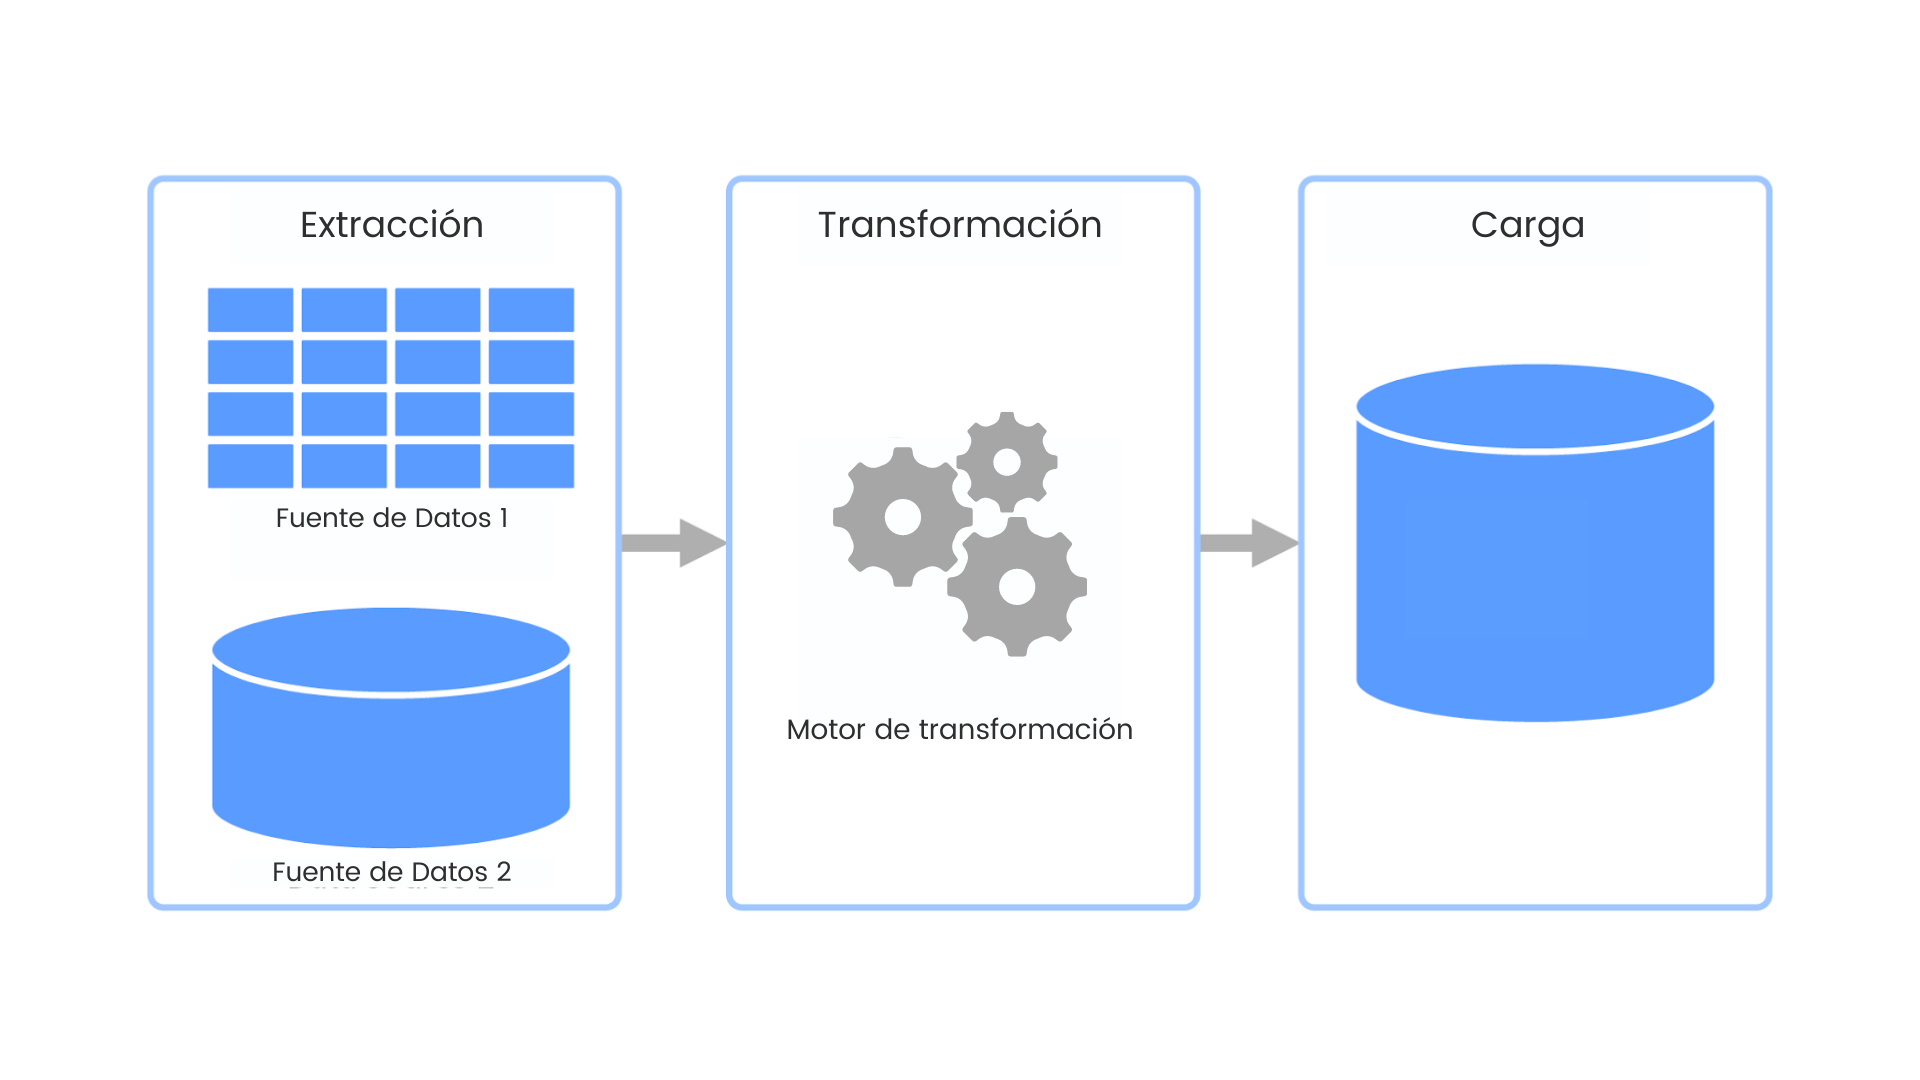
\includegraphics[width=1\linewidth]{img/etl.png}
    \caption{Estructura de un proceso ETL}
    \label{fig:ProcesoETL}\cite{ProcesoETL} 
\end{figure}

\paragraph{Transformación de Datos:}
en esta segunda fase los datos van a ser transformados y limpiados, ya que las herrmaientas que pertenecen a esta parte del proceso ETL permiten: cargar solo ciertas secciones o columnas, modificar tipos de variables, agrupar los datos en rangos preseleccionados o generar nuevos campos a partir de los existentes.

\paragraph{Carga de Datos:}
en la última parte del proceso consiste en que una vez tengamos los datos transformados, estos vayan siendo cargados en el lugar destino que le indiquemos (e.g., ElasticSearch) para que allí sean indexados y gestionados de una manera concreta.

\capitulo{4}{Técnicas y herramientas}

En este apartado se muestran y desarrollan todas las técnicas y herramientas empleadas para completar el estudio y su posterior documentación. Esta sección fundamentalmente se centra en explicar los tres elementos del \textit{stack ELK} que se compone de ElasticSearch, Logstash y Kibana, tal y como indica su acrónimo. ElasticSearch almacena la información proveyendo un acceso eficiente, Logstash la transforma antes de ser almacenada y Kibana la presenta de forma atractiva mediante \textit{dashboards}. 

\section{ElasticSearch}
Este programa de código abierto va a ser la piedra angular y sobre la que van a pivotar el resto de elementos sofware que van a componer las distintas configuraciones a experimentar . Consiste en un motor de búsqueda analítica y distribuida de cara a almacenar todos los datos de un proyecto. \cite{ElasticSearch}

En el presente trabajo se ha empleado el servicio local de Elastic, teniendo que descargar el programa íntegro y operar desde ahi. Se nos ofrece una versión Cloud que promete grandes mejoras en el rendimiento, pero no vimos oportuna su adquisición puesto que el estudio está pensado para herramientas \textit{freeware} sin suponer ningún coste económico.

Funciona como una base de datos estructurada en índices que agrupan colecciones de datos sustituyendo a lo que serían, por ejemplo, tablas de las bases de datos relaciones. Elastic no está enfocado en trabajar con transacciones CRUD, sino en indexar grandes volúmenes de información reduciendo todo lo posible los tiempos de acceso a los datos. Cada índice estructura la información como documentos JSON de manera que cada fila de información quede ordenada y accesible. Desde el apartado \textit{Index Management}, Elastic permite visualizar los diferentes índices presentes en el sistema  (ver ilustración   \ref{fig:indices}).

\begin{figure}
    \centering
    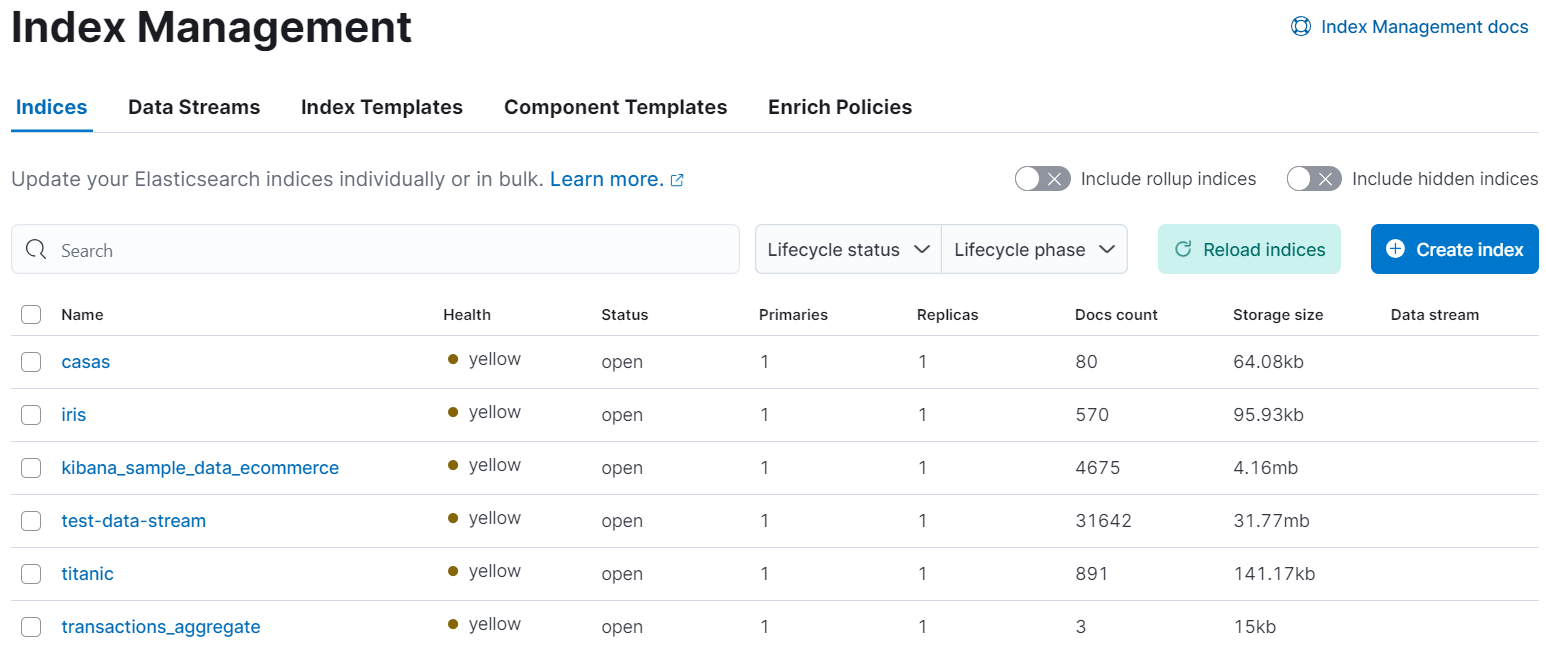
\includegraphics[width=1\linewidth]{img/management.png}
    \caption{Menú principal del \textit{Index Management} de Elastic.}
    \label{fig:indices}
\end{figure}

\section{Logstash}
Actuará como intermediador entre la fuente de datos y Elastic, es decir, cubrirá todo lo relacionado tanto con la parte de transformación de datos como con la de carga de los mismos. Cabe aclarar que se pueden cargar datos en Elastic sin Logstash, pero entonces se cargarían tal y como estén, por lo que todas las transformaciones necesarias tendrán que haberse hecho previamente. 

Logstash permite definir \textit{pipelines} para procesar datos del lado de la fuente de ingesta de datos que permite transformarlos para después enviarlos y cargarlos en el destino indicado (i.e., ElasticSearch) \cite{Logstash}.

Logstash está enfocado tanto a la ingesta de datos, permitiendo cargar datos de múltiples orígenes con compatibilidad con protocolos, como al envío de datos a diversos destinos mediante un \textit{pipeline} configurable.

En este \textit{pipeline}, se pueden realizar modificaciones a los datos que entran. Algunos ejemplos de transformaciones con Logstash pueden ser estos:
\begin{itemize}
    \item El filtro \textit{mutate} permite cambiar nombres de campos, añadir nuevos o eliminar los que se consideren reduntantes. Un ejemplo de su uso es la figura \ref{fig:mutate} en la cuál se realiza un cambio de nombre de un campo, se añade un campo nuevo y se borra un campo.
    \item El filtro \textit{date} permite analizar campos que sean fechas indicándole con que formato están escritas. Un ejemplo de su uso es la figura\ref{fig:date}.
    \item El filtro \textit{csv} permite analizar los campos presentes en un fichero de tipo CSV de manera que divida cada línea en campos indicados. Un ejemplo de su uso es la figura\ref{fig:csv}.

\end{itemize}

\begin{figure}
    \centering
    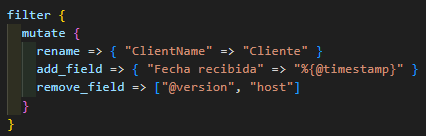
\includegraphics[width=1\linewidth]{img/mutate.png}
    \caption{Ejemplo de uso de filtro \textit{mutate}}
    \label{fig:mutate}
\end{figure}

\begin{figure}
    \centering
    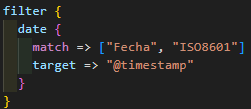
\includegraphics[width=1\linewidth]{img/date.png}
    \caption{Ejemplo de uso de filtro \textit{date}}
    \label{fig:date}
\end{figure}

\begin{figure}
    \centering
    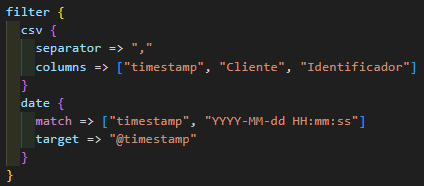
\includegraphics[width=1\linewidth]{img/csv.png}
    \caption{Ejemplo de uso de filtro \textit{csv}}
    \label{fig:csv}
\end{figure}

\paragraph{    }
\paragraph{  }
\paragraph{  }

\section{Kibana}
Por último, la parte de final del stack esta protagonizada por este programa, que se encargará de ejecutar las analíticas de los datos mandados por Logstash a Elastic y de mostrarlos en diferentes \textit{dashboards} con gráficas de datos que nos permitirá generar interacciones que resulten útiles e interesantes \cite{Kibana}.

Kibana permíte administrar los datos presentes en Elastic desde el apartado \textit{Data Views}, facilitando el acceso a los diferentes índices de datos. Un \textit{Data View} consiste en una representación de los datos de un índice para que pueda haber representaciones de los datos en un \textit{dashboard}  (ver ilustración  \ref{fig:dataviews}).

Una vez se accede una \textit{view}, el apartado \textit{Discoverer} es la herramienta que facilita Kibana para poder ver de manera completa la información de los datos presentes en un índice. Se pueden aplicar filtros o clasificaciones para encontrar determinados datos  (ver ilustración   \ref{fig:discoverer}).

Por útlimos, la función principal de Kibana es crear \textit{dashboards} con visualizaciones y demás herramientas sobre los datos presentes en Elatic a través del apartado \textit{Dashboards}, en el cuál se desarrollan tanto la creación como modificación de estos  (ver ilustración \ref{fig:dashboard}).

\begin{figure}
    \centering
    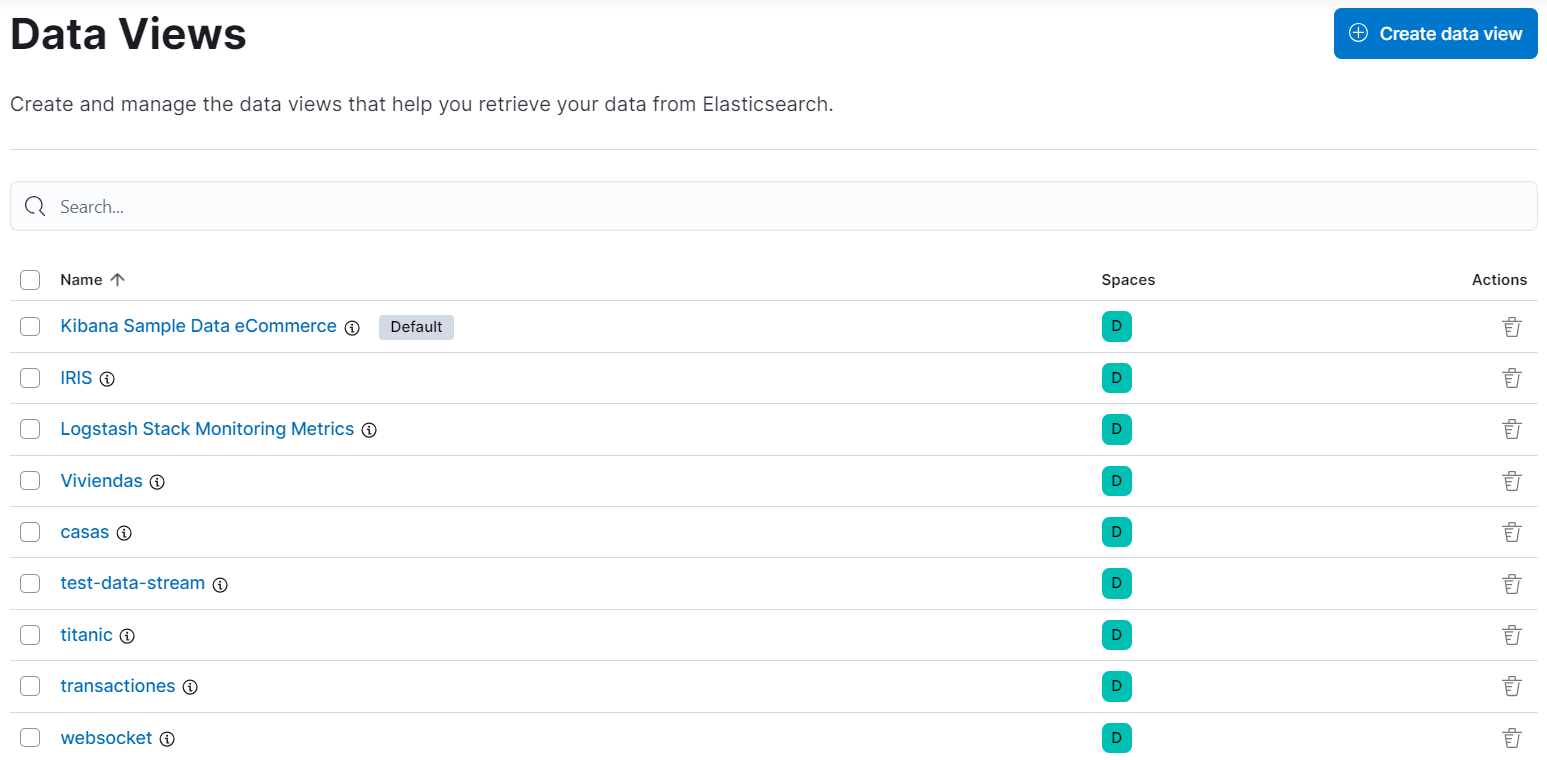
\includegraphics[width=1\linewidth]{img/views.png}
    \caption{Menú principal de los \textit{Data Views} de Kibana.}
    \label{fig:dataviews}
\end{figure}

\begin{figure}
    \centering
    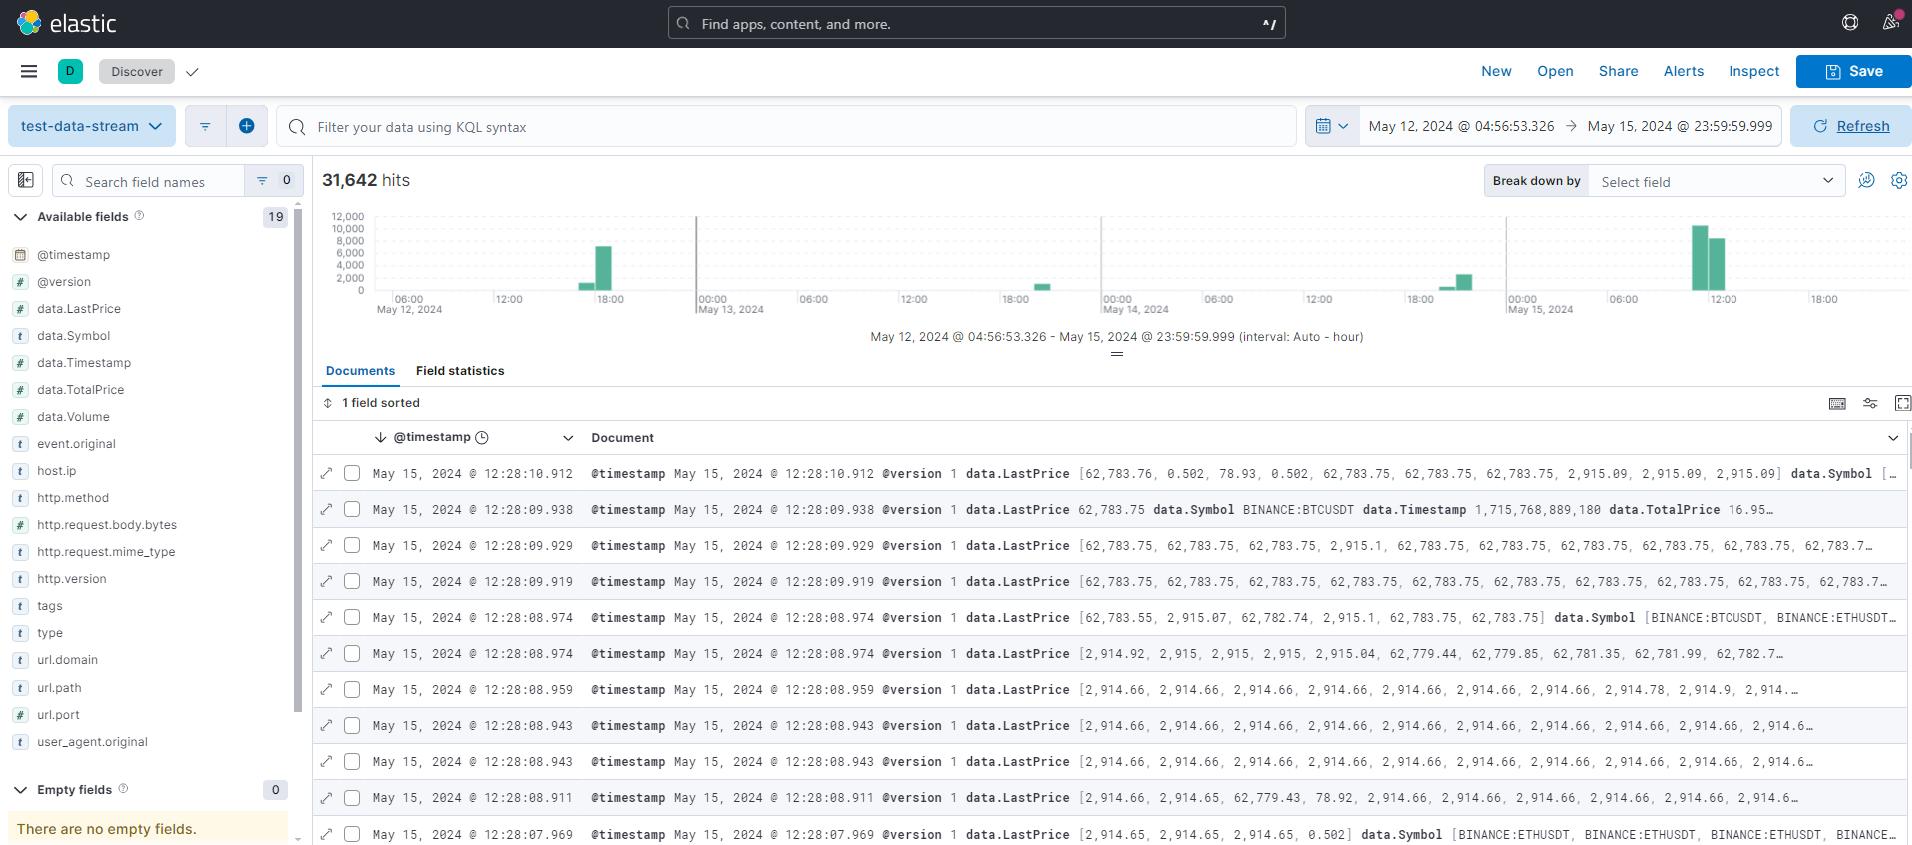
\includegraphics[width=1\linewidth]{img/discoverer.png}
    \caption{Apartado \textit{Discoverer}}
    \label{fig:discoverer}
\end{figure}

\begin{figure}
    \centering
    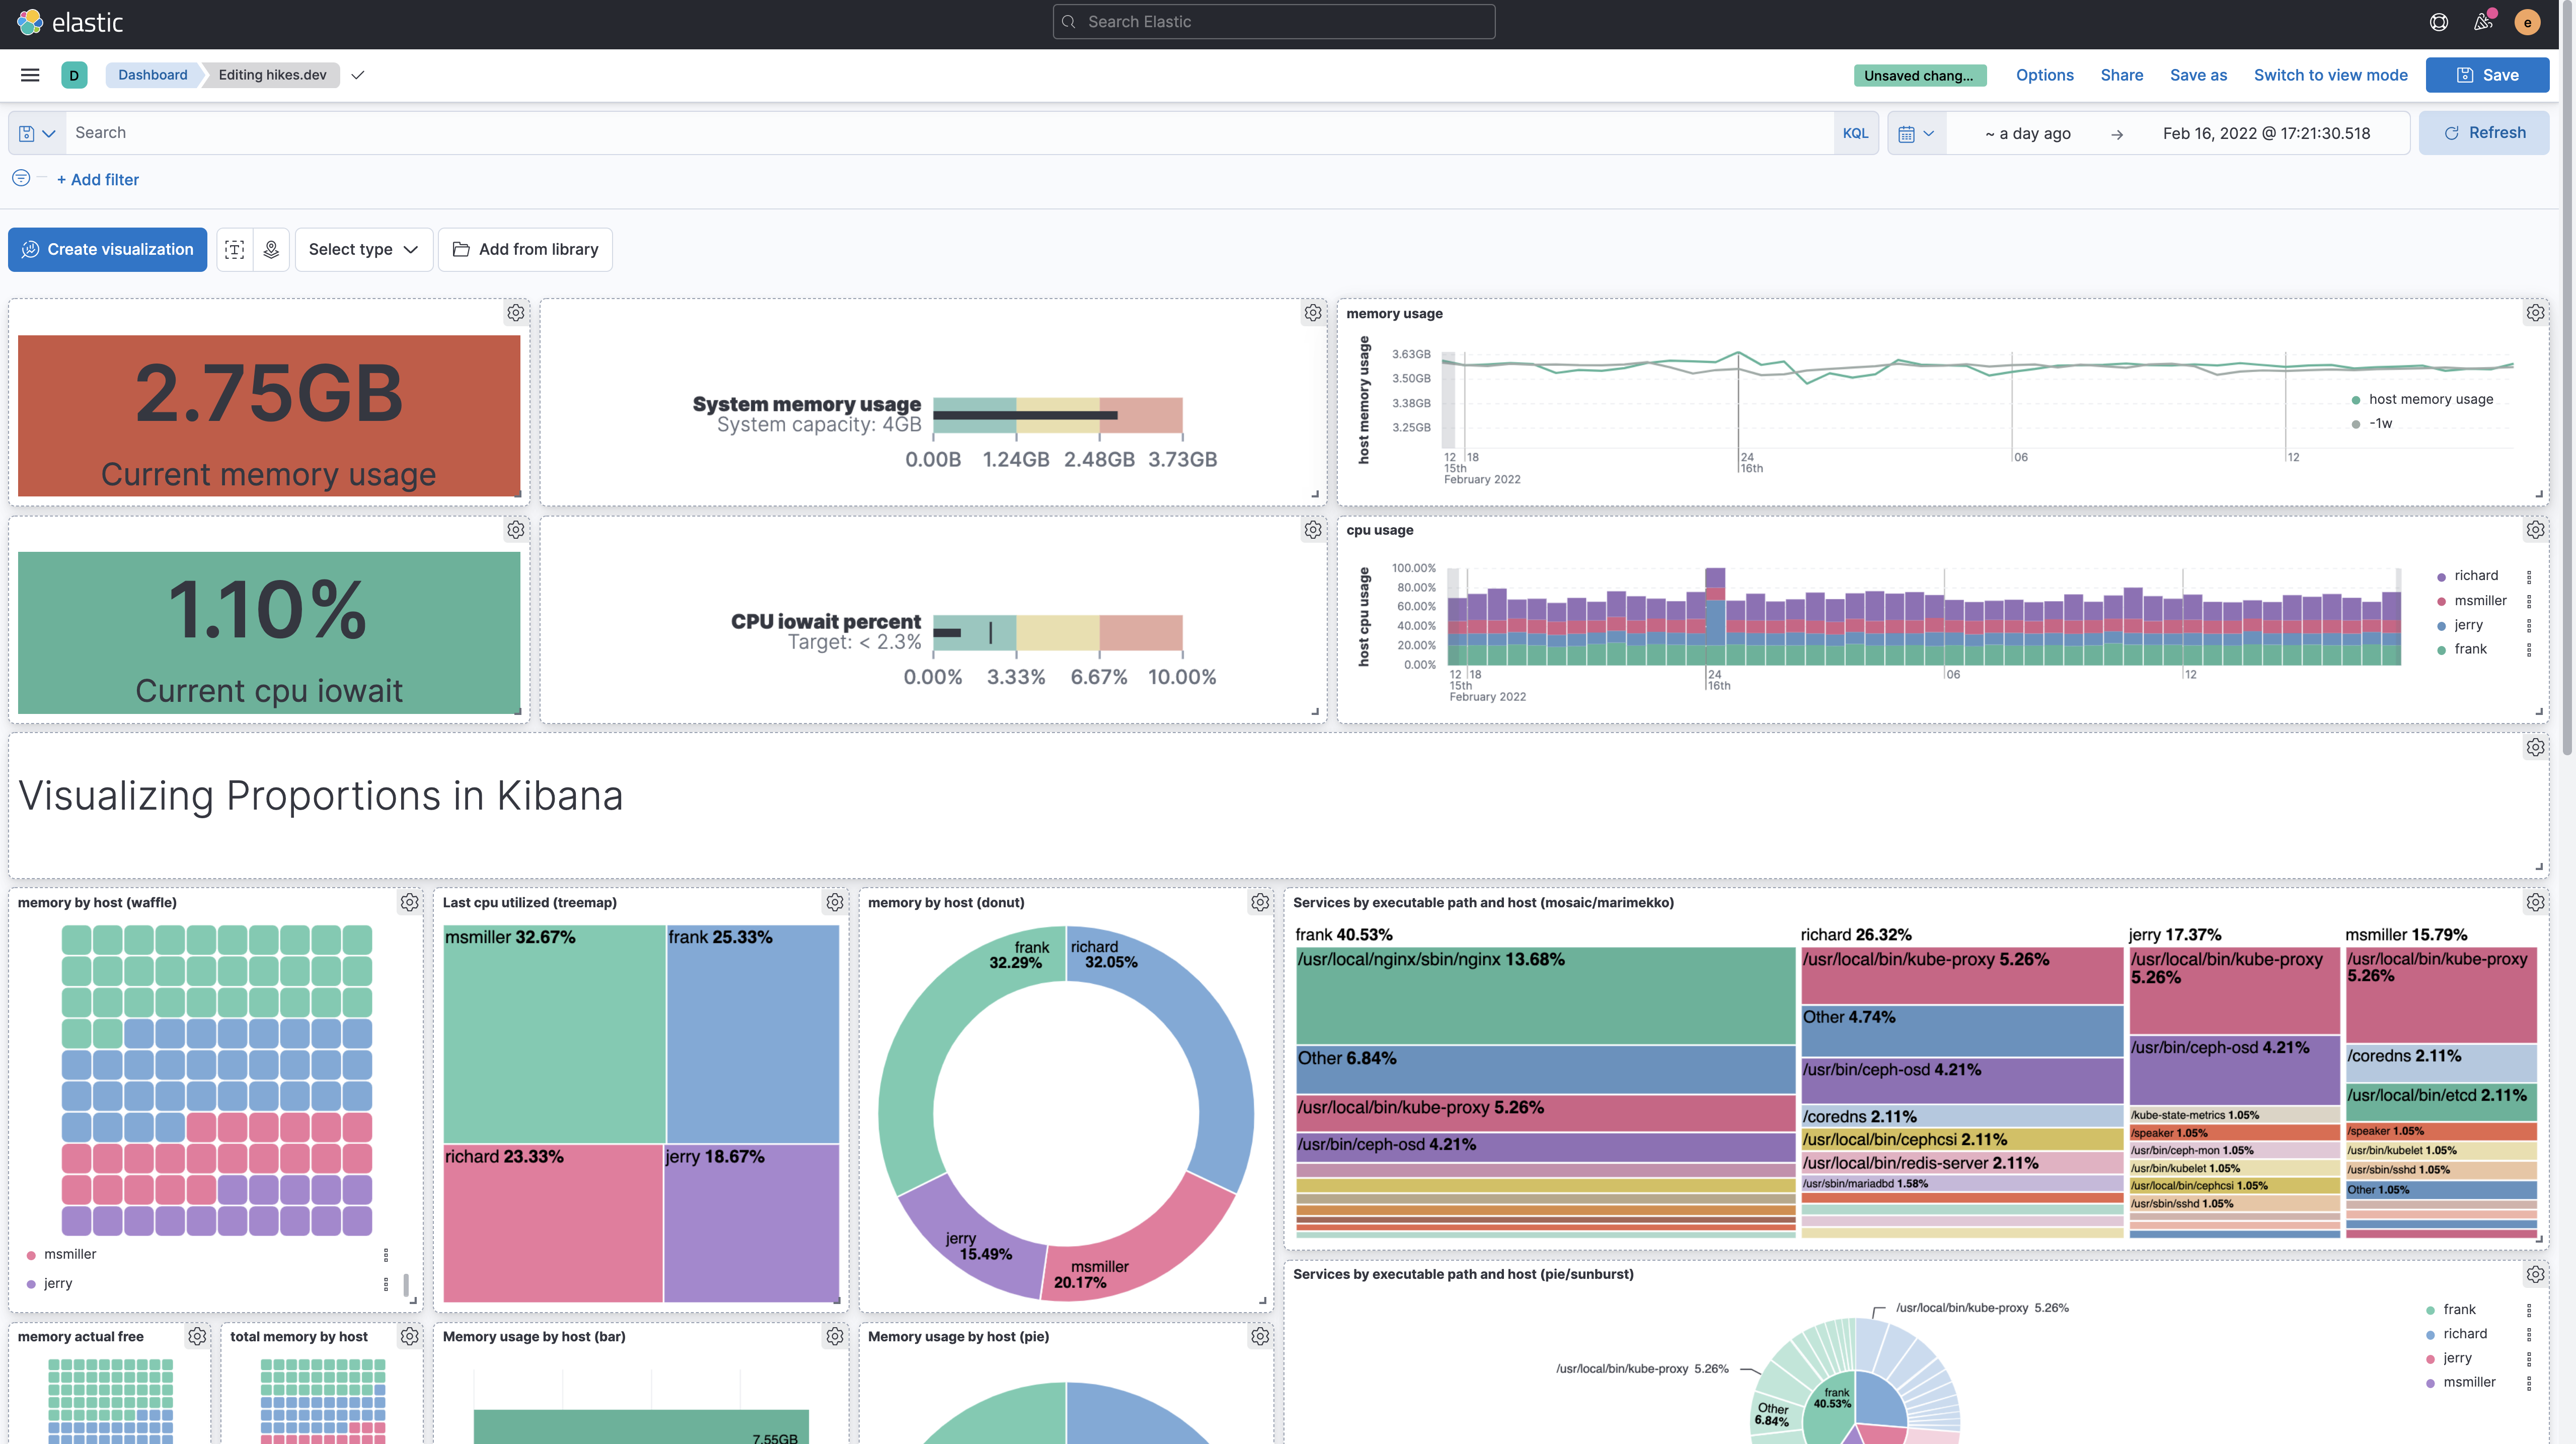
\includegraphics[width=1\linewidth]{img/kibana1.png}
    \caption{Dashboard de Kibana}
    \label{fig:dashboard}
\end{figure}

\section{Miscelánea}

\subsection{Scikit-Learn}
Biblioteca de aprendizaje automático de código abierto para \textit{Python} que permite utilizar algoritmos de clasificación, regresión, clustering y reducción de características a los datos que se le indiquen \cite{scikit}.

\subsection{Jupyter Notebook}
Aplicación web basada en \textit{Python} que se usará para crear y compartir documentos en los que realizamos cálculos computacionales con el resto del entorno de trabajo de los escenarios planteados \cite{jupyter}.

\subsection{Python}
Este lenguaje de programación permite el diseño e implementación de manera sencilla y eficiente de \textit{scripts}, en los cuales se emplean diferentes bibliotecas que utilizaremos para procesar los datos de diferentes maneras. Una vez finalizados son integrados en nuestro ecosistema de trabajo para ofrecer ayuda en distintos escenarios \cite{python}.

\subsection{Visual Studio Code}
Editor de código fuente desarrollado por Microsoft que permite crear, depurar y procesar archivos de código con total soltura. En este proyecto será empleado como apoyo para los diferentes \textit{scripts} de procesamiento de datos realizados \cite{code}.

\subsection{Overleaf}
Editor online de LATEX que permite la edición y exportación de documentos con este formato de manera fácil y rápida. En este proyecto tiene utilidad en la parte de la documentación tanto de la memoria como de los anexos \cite{overleaf}.

\subsection{GitHub}
Este \textit{software} sirve como alojamiento de proyectos, permitiendo modificaciones en el mismo, creaciones de archivos, modificaciones y demás. Será utilizado para mantener un orden en cuánto a la evolución del proyecto \cite{github}.
\capitulo{5}{Aspectos relevantes del desarrollo del proyecto}

En esta sección de la memoria se mostrará las diferentes fases de maduración y evolución por las que ha pasado el proyecto, haciendo especial hincapié en las dificultades encontradas a la hora de afrontar distintas tareas. También se mostrarán los resultados obtenidos en el estudio.

\section{Evolución temporal}

\subsection{Inicio y motivación}

A principios de curso, tuve la oportunidad de realizar las prácticas curriculares en la consultoría informática local CSA, más concretamente en el departamente de Business Intelligence. Ahí estuve trabajando durante meses con distintas herramientas de la categoría ETL que me resultaron prácticas e interesantes. Por lo que una vez finalizadas las prácticas, le propuse a mi tutor de las mismas la posibilidad de realizar mi trabajo de fin de grado sobre algo relacionado con el tratamiento de datos. Y así llegamos a la conclusión de empezar a trabajar con las herramientas ElasticSearch, Kibana y Logstash, que cumplían el papel de las tres fases de un proceso ETL.

La intención en este proyecto siempre fue desde el principio un estudio de estas herramientas ELK en el que se representerán situaciones que pudieran ocurrir en un entorno real. Por lo que desde un inicio, se pensó en plantear distintos escenarios en función de la manera en la que se ingestaban los datos.

El primer interrogante que se planteó por parte del tutor, Jesus Manuel Maudes Raedo, fue el de investigar que posibilidades ofrecía Logstash a la hora de ingestar, filtrar y exportar datos. En un principio, la idea se antojaba sencilla pero debido a que estos programas son novedosos y no han tenido tanto impacto (aún) como otros como puede ser PowerBI, la documentación presente en Internet sobre conceptos relacionados con este programa era escasa y en su mayoría en lengua anglosajona. Por lo que se comenzó desde lo más básico, tutoriales y guías tanto de plataformas como YouTube, como de las páginas oficiales de Elastic. 

La familiarización con el programa Logstash llevó un gran lapso de tiempo, por lo que se compaginó con investigar el funcionamiento de los plugins que ofrece Elastic desde su \textit{marketplace}, comprender como se podía realizar integraciones con \textit{Python} en el ecosistema Elastic, y estudiar la posibilidad de integrar \textit{machine learning} en el análisis de los datos, y este fue el siguiente punto que se tocó en profundidad.

En este periodo, se completó el primero de los escenarios a analizar y más sencillo, el de importar directamente un fichero de tipo CSV a Elastic. El fichero elegido fue uno que incluía datos sobre los pasajeros del Titanic y que ofrecia la posibilidad de mostrar diferentes herramientas que nos ofrece Kibana a la hora de mostrar los datos.
También se analizó un ejemplo de datos que nos ofrece Elastic que permite explotar al máximo las capacidades de analisis de Kibana. Se trata de los datos de una empresa electrónica que se dedica al comercio de artículos, y gracias a este escenario se pudo comprender con mayor facilidad el funcionamiento de Kibana de cara a desarrollar los siguientes escenarios que se avecinaban.

\paragraph{}
\paragraph{}
\paragraph{}
\paragraph{}
\paragraph{}


\subsection{Cronología de los experimentos}

\subsubsection{Machine Learning}

Habiendo pasado ya un mes desde el comienzo del estudio, la posibilidad de integrar análisis de datos con \textit{machine learning} se antojaba fundamental, pues a priori era una función de pago que ofrece Elastic, por lo que esa vía de integración quedó descartada.

Se introdujo la idea de trabajar con la biblioteca de aprendizaje automático de código abierto \textit{Scikit-Learn}. Para el segundo sprint del proyecto, se giró entorno al estudio, comprensión e investigación de esta biblioteca que se consiguió integrar a través la herramienta \textit{Jupyter Notebook}, en la que se realizaron distintos scripts de pruebas para comprender el funcionamiento de los algoritmos de clasificación, regresión, clustering y reducción de características sobre el \textit{dataset} Iris, un popular conjunto de datos empleado como ejemplo de la utilidad del \textit{machine learning} en el análisis de los mismos. Este conjunto de datos ya lo tenemos almacenado en Elastic, y es desde donde lo cargamos al script para poder trabajar sobre esa información. Una vez los los algoritmos los han procesado, estos datos son ingestados en índices indivuales en ElasticSearch. Una vez se hubo finalizado la carga de los resultados, estos fueron expuestos en un \textit{dashboard} en la herramienta visual Kibana. 

Al no haber cursado la asignatura optativa de Minería de Datos, este proceso de aprendizaje fue costoso y ocupó un gran período de tiempo hasta que se comprendieron de manera correcta los conceptos tratados.

También se mencionó la posibilidad de realizar funciones como Map Reduce en algún momento del ETL, y se dedicó un tiempo a investigar en qué momento y en qué herramienta era más óptimo implementar esta función. 

\paragraph{}
\paragraph{}
\paragraph{}
\paragraph{}
\paragraph{}

\subsubsection{Data Streams}

Con lo mencionado anteriormente se finalizó el segundo sprint y dieron comienzo los dos siguientes, en los que la misión principal fue la de estudiar el funcionamiento de los \textit{streams} de datos, cómo funcionan y de qué forma los podemos ingestar en Elastic.

El tutor de este proyecto proporcionó distintas fuentes para encontrar \textit{streamings} de datos con los que poder experimentar y estudiar las posibilidades reales que ofrecen. Se continuó por un repositorio de GitHub de nombre \href{https://github.com/ColinEberhardt/awesome-public-streaming-datasets}{awesome public streaming datasets} en el que se incluían distintas interfaces via \textit{WebSockets} de \textit{data streams}. El problema venia dado cuando queríamos ingestar estos \textit{streamings} con Elastic, ya que bastantes de las APIs que se ofrecían eran complejas, y las que no, ofrecían envios de datos muy básicos. A todo esto se le suma que no habiendo cursado la asignatura de Sistemas Distribuidos, en la cuál se estudia el funcionamiento de los \textit{WebSockets} detenidamente, me supuso un mayor tiempo para la compresión de estos conceptos.

Por lo que se optó por una opción que era gratuita y satisfacia en gran parte los requisitos que se pedían: la \textit{RESTful API} y \textit{WebSocket} de la empresa de operaciones de criptomonedas \textbf{Finnhub}.

Gracias a la guía que presentan su \href{https://finnhub.io/docs/api/websocket-trades}{página web}, y los diferentes tutoriales y documentación presente en Internet, se consiguió desarrollar un script en Python que se suscribiese al \textit{stream} de datos y mandará los datos directamente a Elastic, sin realizar ninguna operación intermedia, completando así otro de los escenarios tratados.

En vista de que existía la posibilidad de realizar alguna manipulación o transformación a los datos originales que Finnhub mandaba, se optó por generar un script que modificará el nombre de las variables y mandará a Logstash los datos del \textit{stream} para poder realizar más filtros desde allí. El envío de datos del script a Logstash se realiza a través del protocolo de red HTTP, a través del puerto 8080 más concretamente.

Una vez los datos llegan a Logstash, se les realiza unas modificaciones, omitiendo el envío de campos vacíos, modificando el tipo de las variables para que sean legibles por Elastic, y generando nuevos campos en base a los originales relizando operaciones sobre ellos. Una vez que los filtros se realizan los datos procesados por Logstash son mostrados por pantalla y enviados a Elastic para que desde allí puedan ser ilustrados y expuestos a través de Kibana, dando fin así a otro de los posibles escenarios analizados.

Cabe remarcar que al encontrar dificultades en el envío de datos a través de las fuentes del repositorio mencionado, se estudió paralelamente la posibilidad de mandar los datos con la herramienta \textit{Filebeat}, la cuál ofrece una integración sencilla con Elastic pero teniendo acceso a \textit{streamings} de datos más complejos. Por lo que añadir esta opción hubiera sido aumentar la carga de trabajo, por lo que se deja como posible mejora de cara a trabajos futuros.

\section{Resultados del estudio}

\subsection{Introducción}
Una vez maduradas las posibilidades que ofrece el sistema ELK, se ha decidido estructurar este apartado en varios, en función de las conclusiones sacadas. Se hará hincapié en los conceptos teóricos mencionados previamentes como pueden ser MapReduce o Machine Learning entre otros.

\subsection{ELK con Elastic en la nube}

Elastic ofrece la versión de trabajo \textit{cloud}, en la que se dispone de un espacio de almacenamiento para los distintos índices de datos de manera que se puedan trabajar con ellos desde distintas ubicaciones. Esta funcionalidad es ofrecida pagando un precio efectivo, por lo que no lo contemplamos como posibilidad de trabajo. Pero de forma gratuita, Elastic pone a servicio del usuario diversas fuentes de datos en su nube para poder experimentar y aprender a sacar el máximo potencial tanto a ElasticSearch como a Kibana.

Tras evaluar la situación, se llegó a la conclusión de que los datos utilizados en los diferentes escenarios permitían a Kibana mostrar parte de su potencial, pero no todo. Por lo que para mostrar la herramienta al completo se utilizaron datos que nos ofrece Elastic a modo de ejemplo.

En este caso, se eligieron los datos sobre un \textit{e-commerce} el cuál recibe pedidos de todo el mundo y de distintos tipos. Permitiendo así poder mostrar visualizaciones de mapas, histogramas y demás funciones avanzadas, como pueden ser los distintos gráficos de líneas para evaluar la evolución de los gastos por categorías o gráficos de barras en lo que se muestra la evolución de las ganancias a lo largo de un marco temporal.

\begin{figure}
    \centering
    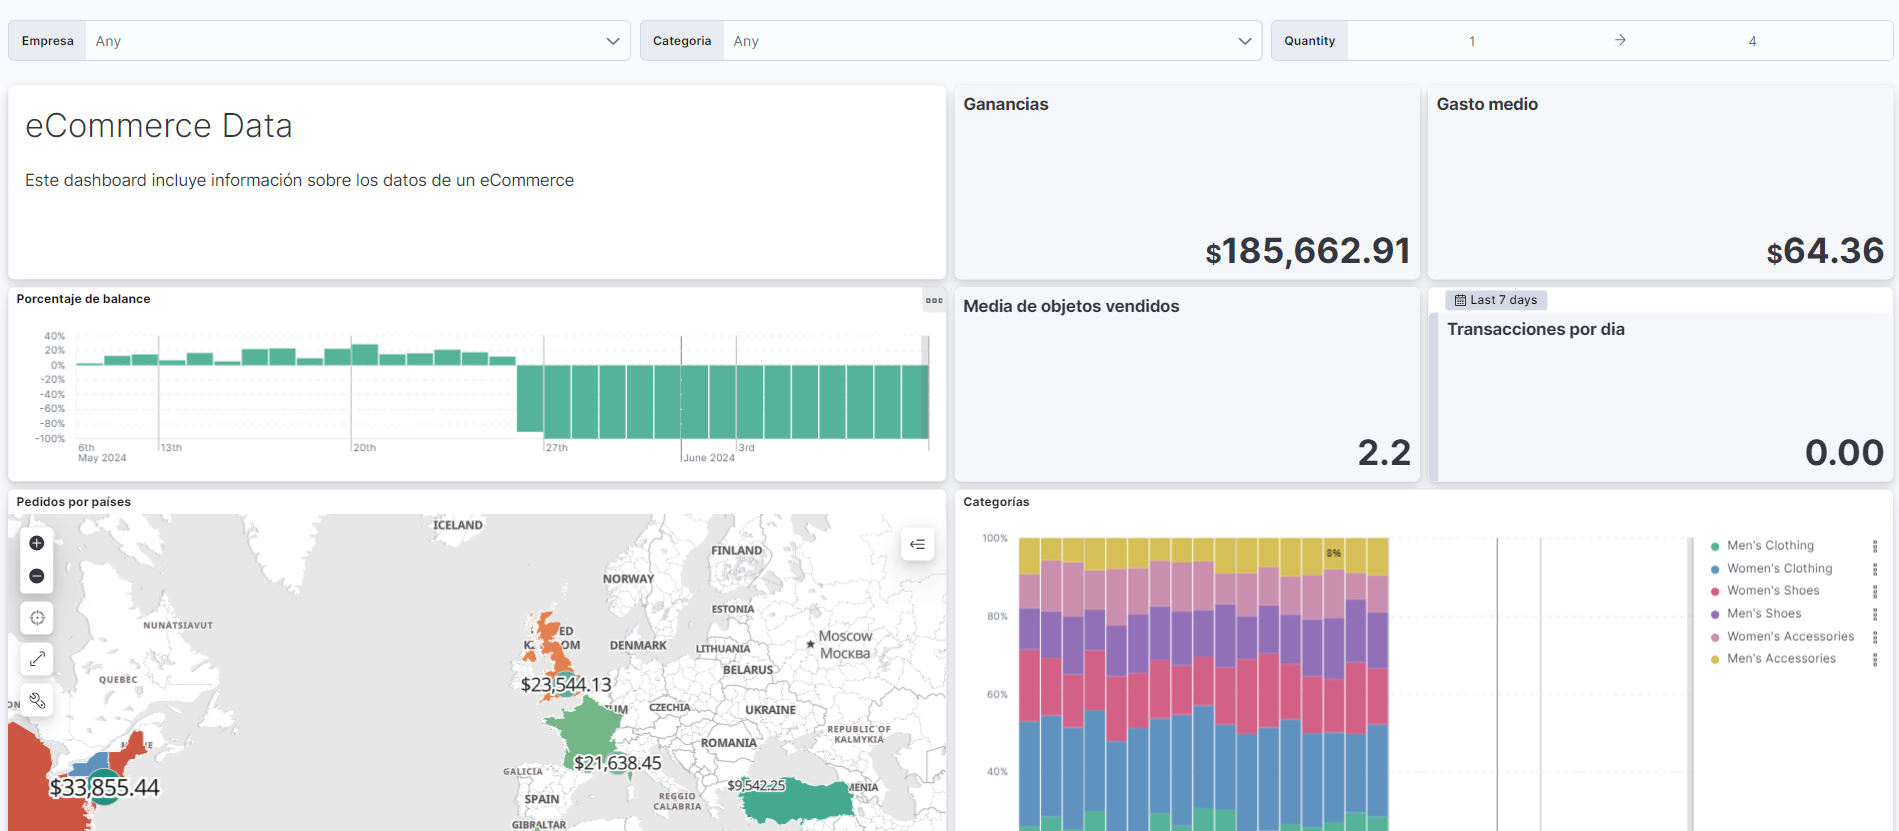
\includegraphics[width=1\linewidth]{img/escenario6.png}
    \caption{Dashboard final}
    \label{fig:escenarioNube}
\end{figure}

\paragraph{ }
\paragraph{ }
\paragraph{ }
\paragraph{}
\paragraph{}
\paragraph{}
\paragraph{}
\paragraph{  }
\paragraph{  }
\paragraph{  }
\paragraph{  }
\paragraph{  }


\subsection{Escenarios de ingesta de datos}

En este apartado se hará un desglose de los diferentes escenarios de ingesta de datos de diversas fuentes sobre los que se ha trabajado en este estudio incluyendo su desarrollo y resultados finales obtenidos.

\subsubsection{Escenario 1: ingesta desde fichero en Elastic}
Este primer escenario es el más simple de todos, consiste en la importación de un fichero local a Elastic a través del servicio de importación de datos básico que se ofrece.

El archivo que se va a analizar recibe el nombre de \textit{titanic.csv}, es un archivo de valores separados por comas que muestra datos sobre los pasajeros que formaban parte de la tripulación del hundido barco \textit{Titanic}.
Es un archivo interesante como punto de partida para entender el funcionamiento de las herramientas software empleadas.

Teniendo este archivo en el sistema local, en el apartado que dice "import from file", y desde ahi se selecciona el mencionado CSV. Una vez que lo seleccionado, Elastic cargará los datos y se podrán visualizar desde la pestaña \textit{Discover}, en la que aparecerán las filas del fichero. Desde aquí se pueden clasificar y filtrar de manera que se pueda comprobar que los datos han sido cargados correctamente.

Una vez tenemos los datos cargados, ya se puede crear el \textit{Dashboard} pertinente accediendo a la pestaña \textit{Visualize} y desde aquí a \textit{Dashboard}. Una vez ahí, se seleccionará cuál es la fuente que proveerá de datos las visualizaciones, seleccionamos la del archivo que se acaba de importar, y ya se podrá empezar a generar visualizaciones.

La estructura básica estará formada por un texto descriptivo del \textit{dashboard} en formato Markdown incluyendo datos del autor, así como descripciones de las distintas visualizaciones presentes. Este elemento es fundamental en todo \textit{dashboard} cumpliento el papel de introducción a la hora de la toma de contacto con el contexto de las visualizaciones.

En el \textit{dashboard} resultante se han añadido gráficos de las edades  (ver ilustración  \ref{fig:barras1}), los géneros, métricas  (ver ilustración  \ref{fig:metricas1}), y gráficos de donut  (ver ilustración  \ref{fig:donut1}) en función de la clase del pasajero, la cuál se puede filtrar en función de lo que interese desde la barra superior dónde están presentes los diferentes filtrados que se pueden hacer por género del pasajero, edad de los mismos, por que puerta de embarque accedieron, la clase de su billete o si sobrevivieron  (ver ilustración  \ref{fig:escenario1}).

\begin{figure}
    \centering
    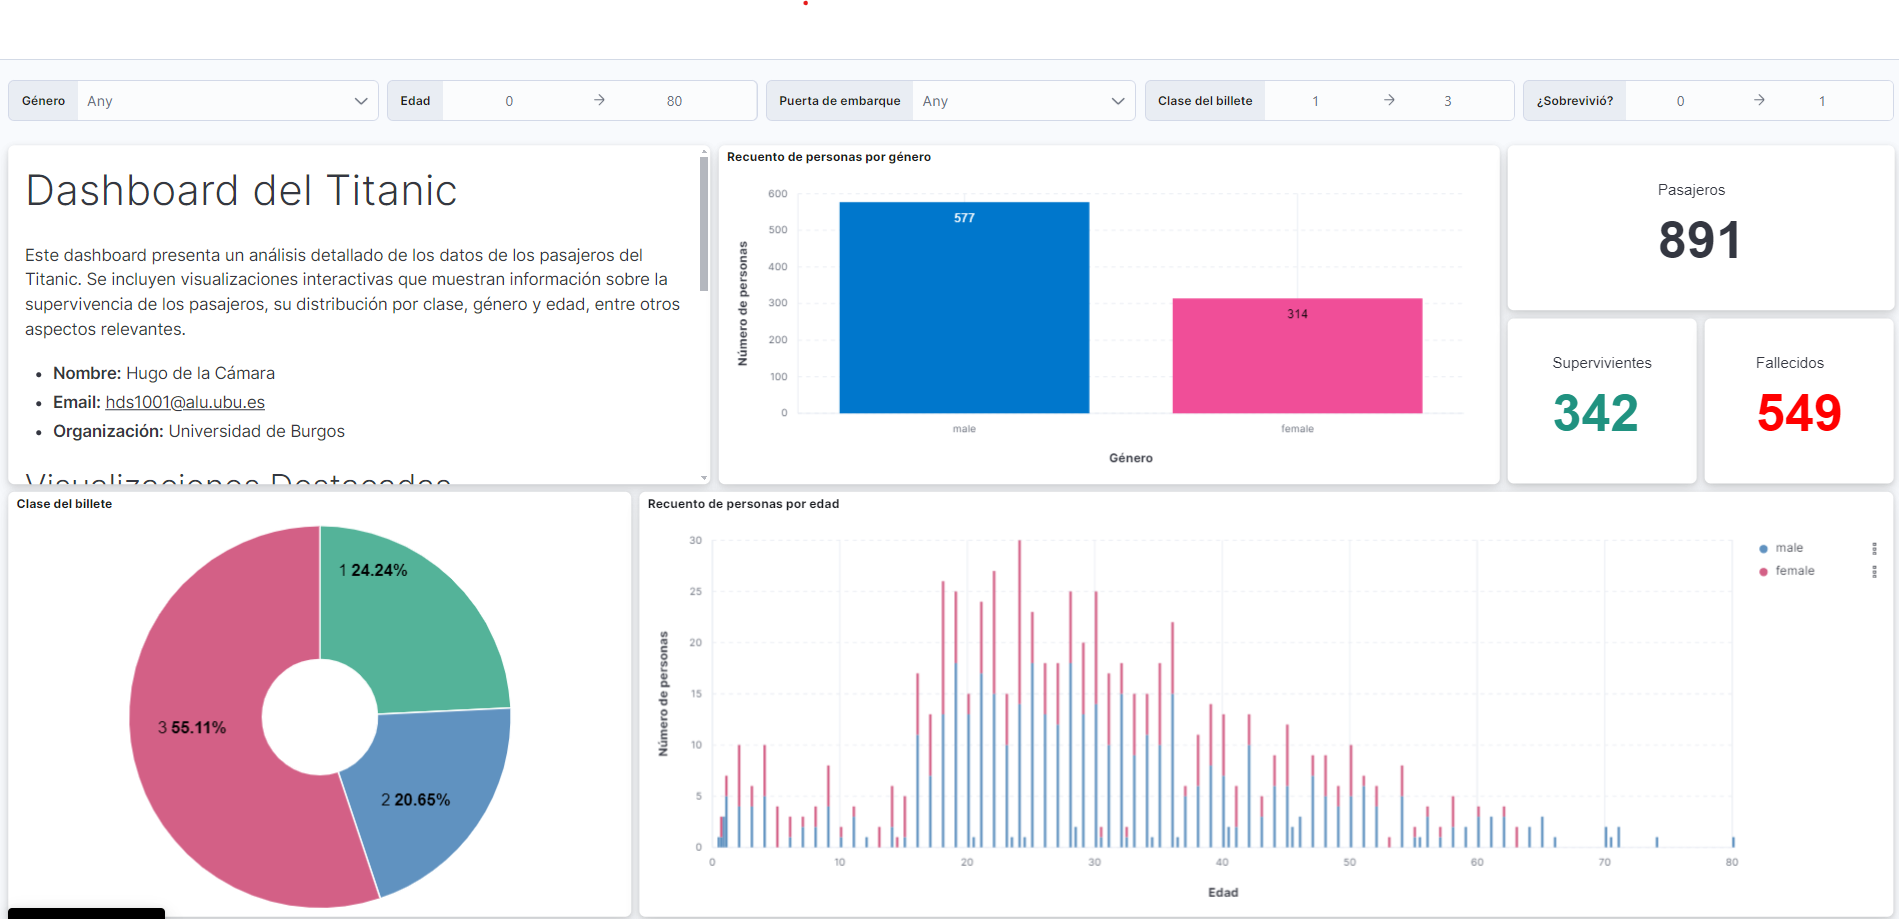
\includegraphics[width=1\linewidth]{img/escenario1.png}
    \caption{Dashboard final del primer escenario}
    \label{fig:escenario1}
\end{figure}

\begin{figure}
    \centering
    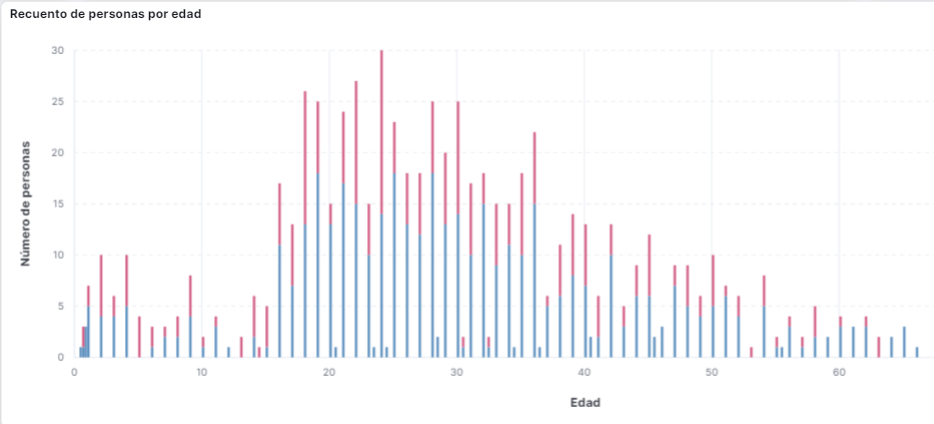
\includegraphics[width=1\linewidth]{img/edades.png}
    \caption{Gráfico de barras por edades y género}
    \label{fig:barras1}
\end{figure}


\begin{figure}
    \centering
    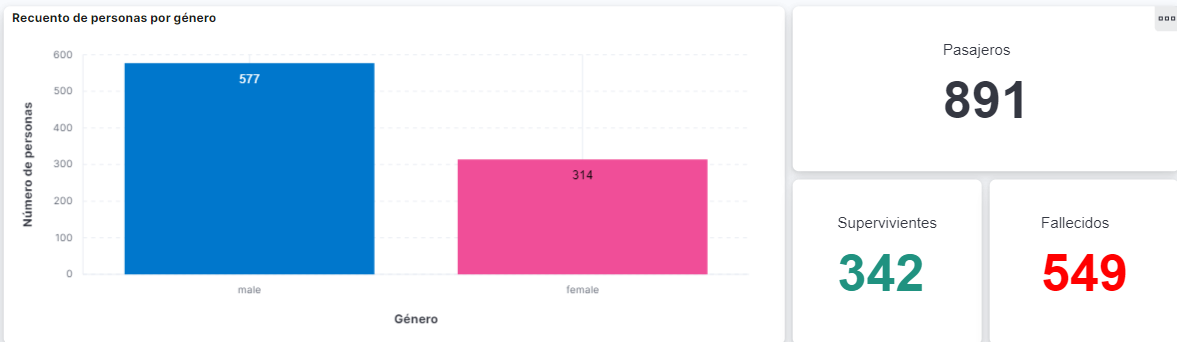
\includegraphics[width=1\linewidth]{img/graficos1.png}
    \caption{Métricas en función del filtrado}
    \label{fig:metricas1}
\end{figure}

\begin{figure}
    \centering
    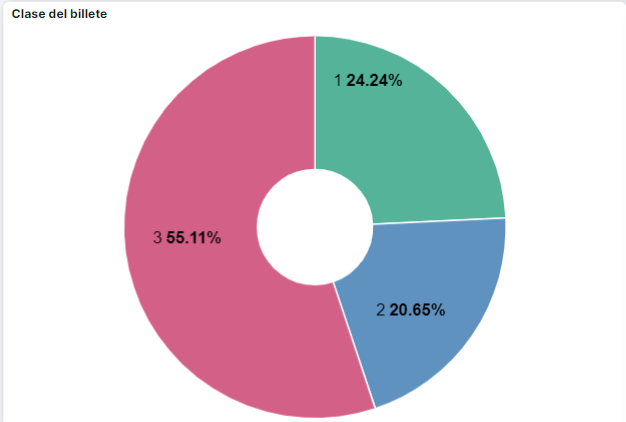
\includegraphics[width=1\linewidth]{img/donut.png}
    \caption{Gráfico de donut en función de la clase del billete}
    \label{fig:donut1}
\end{figure}

\paragraph{}
\paragraph{}
\paragraph{}
\paragraph{}
\paragraph{}
\paragraph{}
\paragraph{}
\paragraph{}

\subsubsection{Escenario 2: ingesta desde fichero con Logstash}

Este segundo caso, es una modificación del primero, lo que se pretende es importar un archivo presente en el sistema en Logstash, realizarle una serie de modificaciones y cargar esos datos tratados en Elastic para poder visualizarlos en Kibana.

El archivo sobre el que se va a trabajar es uno de tipo \textit{log} que indica las diferentes viviendas ofertadas en una inmobiliaria, incluyendo campos como el número de la casa, la ciudad en la que se ubican, el barrio en el que se encuentra, el precio de la misma, el número de habitaciones que tiene, el número de baños disponibles y los metros cuadrados de la vivienda.

Para trabajar con logstash, se necesita un archivo de configuración para que éste entienda lo se le pide que haga. Este archivo es de tipo \textit{.conf} e incluye 3 apartados:
\begin{itemize}
    \item \textbf{Input}: ruta hacia el archivo que se quiere leer
    \item \textbf{Filter}: operaciones a realizarle a estos datos
    \item \textbf{Output}: salida por pantalla de los datos mandados a Elastic una vez son tratados.
\end{itemize}

En este escenario se le va a dar toda la relevancia al apartado \textit{filter} del fichero de configuración  (ver ilustración   \ref{fig:filter}), que va a ser en el que se realizan las transformaciones de los datos. 

\begin{figure}
    \centering
    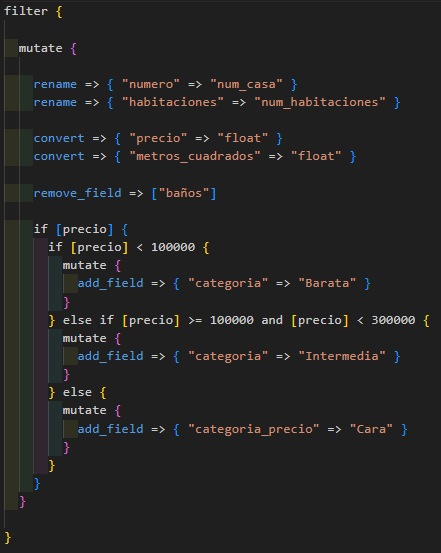
\includegraphics[width=1\linewidth]{img/filter.png}
    \caption{Sección filter del archivo de configuración.}
    \label{fig:filter}
\end{figure}

La primera operación que se va a realizar es la de modificar el nombre de los campos \textit{numero} por \textit{num casa} y de \textit{habitaciones} por \textit{num habitaciones} con la función \textit{rename}  (ver ilustración  \ref{fig:rename}), la cuál permite cumplir esta orden. Esto es de gran utilidad cuándo el nombre de algún campo no deja claro la información que éste ofrece.

\begin{figure}
    \centering
    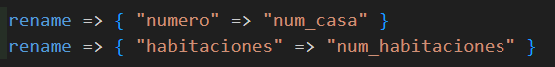
\includegraphics[width=1\linewidth]{img/rename.png}
    \caption{Función que renombra los campos indicados}
    \label{fig:rename}
\end{figure}

La siguiente transformación que se ha aplicado es la de cambiar los tipos de los campos \textit{precio} y \textit{metros cuadrados} con la función \textit{convert}  (ver ilustración  \ref{fig:convert}), la cuál es de gran ayuda cuando los campos que se van a mandar a Elastic no poseen un tipado que permita el correcto procesamiento de la información.

\begin{figure}
    \centering
    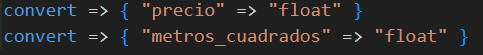
\includegraphics[width=1\linewidth]{img/convert.png}
    \caption{Función que convierte los tipos de los campos indicados}
    \label{fig:convert}
\end{figure}

La tercera operación aplicada en este filtro va a consistir en la eliminación del campo \textit{baños} con la función \textit{remove field}  (ver ilustración  \ref{fig:remove}), la cuál permite eliminar del mensaje final mandado a Elastic contendido que no se considere oportuno o que carece de relevancia.

\begin{figure}
    \centering
    
\includegraphics[width=1\linewidth]{img/remove.png}
    \caption{Función en la que se elimina el campo \textit{baño}}
    \label{fig:remove}
\end{figure}
\paragraph{}

La última transformación es una discretización en función del campo \textit{precio} de cada vivienda  (ver ilustración  \ref{fig:discre}). En ella se indica la creación de un nuevo campo para cada registro llamado \textit{categoria}, en el cuál si la vivienda tiene un precio menor de 100000 será considerada de categoría barata, si el precio oscila entre 100000 y 300000 será considerada de categoría intermedia y si excede la última cantidad será catalogada como cara.

\begin{figure}
    \centering
    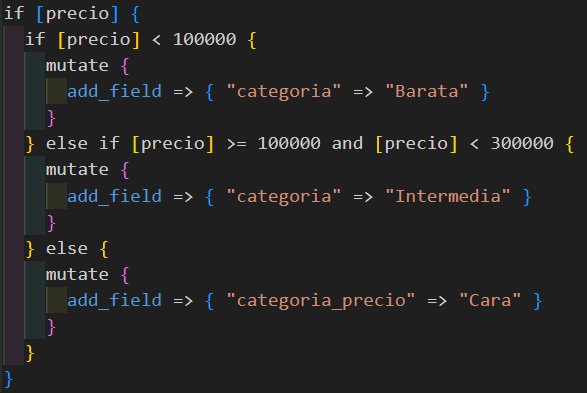
\includegraphics[width=1\linewidth]{img/discretizacion.png}
    \caption{Función en la que se discretiza en función del precio de la vivienda}
    \label{fig:discre}
\end{figure}

Una vez ejecutado Logstash, a Elastic le llega un índice con toda la información que se ha procesado en el filtro. Y una vez se tienen los datos en el entorno, podemos generar el \textit{dashboard}  (ver ilustración  \ref{fig:dashboard2}) para mostrar toda la información.

En este tablero se han incluído visualizaciones como un gráfico de barras en el que se muestra información sobre el número de viviendas por categoría de precio clasificada  (ver ilustración  \ref{fig:barrasViv1}), también una métrica y una tabla que muestran el número total de viviendas  (ver ilustración  \ref{fig:metrica2}), un gráfico de donut mostando el porcentaje de las viviendas que pertenecen a cada ciudad y barrio  (ver ilustración  \ref{fig:donut2}), un gráfico de árbol que muestra la media de metros cuadrados de la vivienda por ciudad  (ver ilustración  \ref{fig:treemap2}) y un gráfico de barras apiladas que muestra el número de viviendas y el número de habitaciones medio por barrio  (ver ilustración  \ref{fig:barrasViv2}).

\begin{figure}
    \centering
    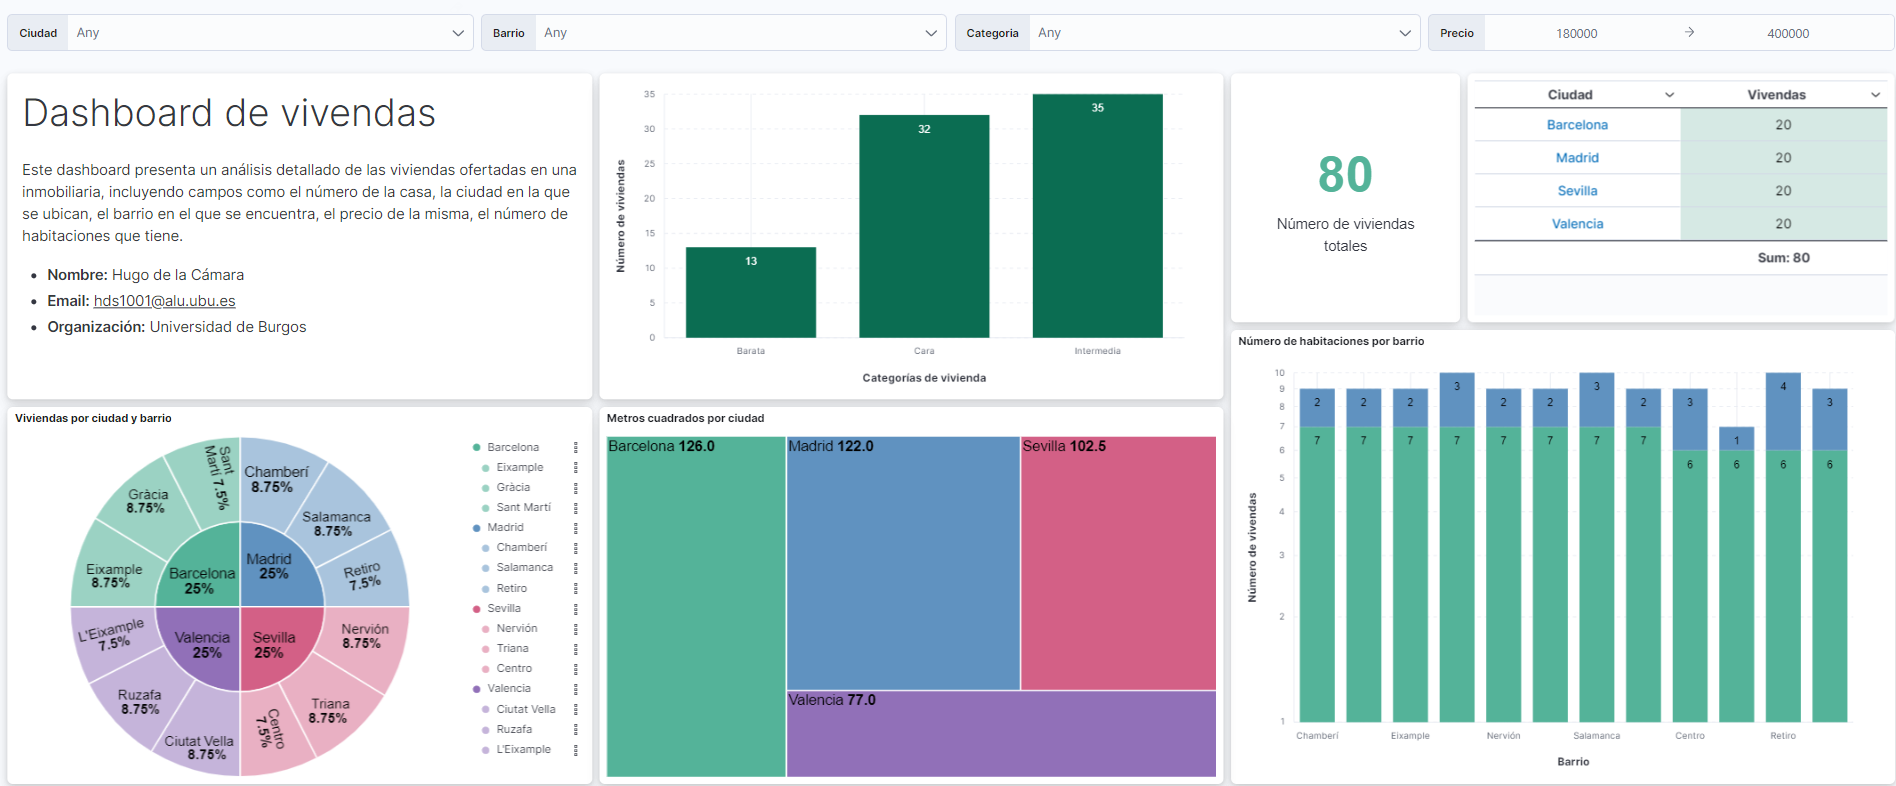
\includegraphics[width=1\linewidth]{dashViviendas.png}
    \caption{Dashboard final del escenario 2}
    \label{fig:dashboard2}
\end{figure}

\begin{figure}
    \centering
    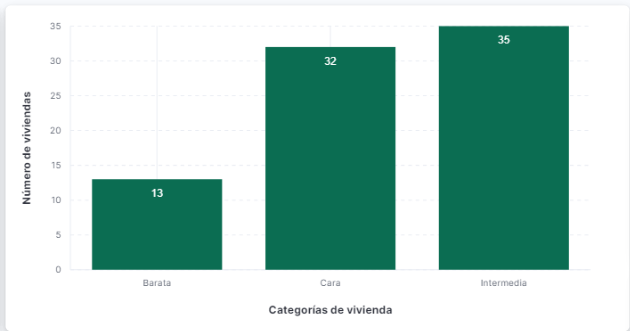
\includegraphics[width=1\linewidth]{img/barrasViv.png}
    \caption{Gráfico de barras del número de viviendas por categoría de precio.}
    \label{fig:barrasViv1}
\end{figure}

\begin{figure}
    \centering
    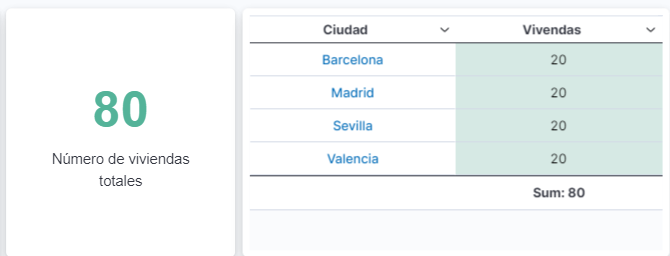
\includegraphics[width=1\linewidth]{img/metricaViv.png}
    \caption{Métrica y tabla del número de viviendas.}
    \label{fig:metrica2}
\end{figure}

\begin{figure}
    \centering
    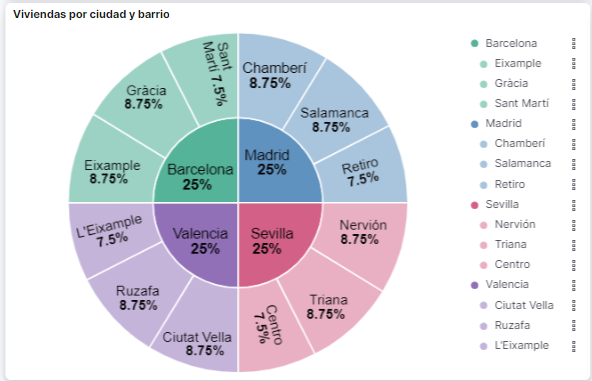
\includegraphics[width=1\linewidth]{img/donutViv.png}
    \caption{Gráfico de donut que muestra el porcentaje de viviendas por ciudad y barrio.}
    \label{fig:donut2}
\end{figure}

\begin{figure}
    \centering
    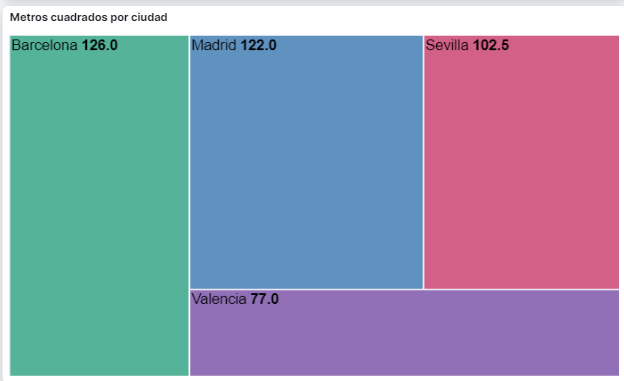
\includegraphics[width=1\linewidth]{img/graficoViv.png}
    \caption{Gráfico de árbol que muestra la media de metros cuadrado por ciudad.}
    \label{fig:treemap2}
\end{figure}

\begin{figure}
    \centering
    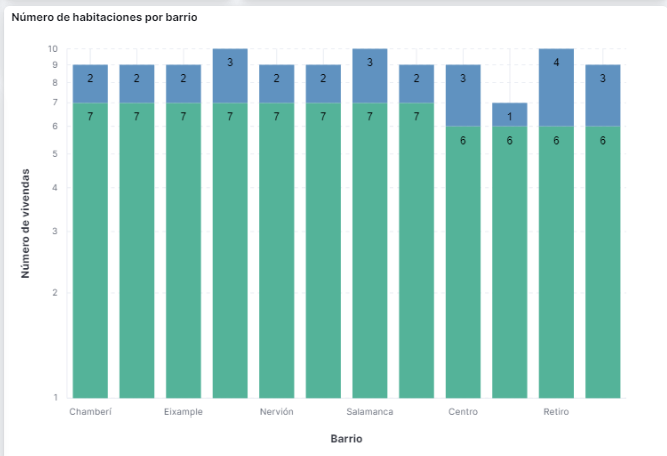
\includegraphics[width=1\linewidth]{img/barras2Viv.png}
    \caption{Gráfico de barras que muestra el número de habitaciones y de viviendas por barrio.}
    \label{fig:barrasViv2}
\end{figure}

\begin{figure}
    \centering
    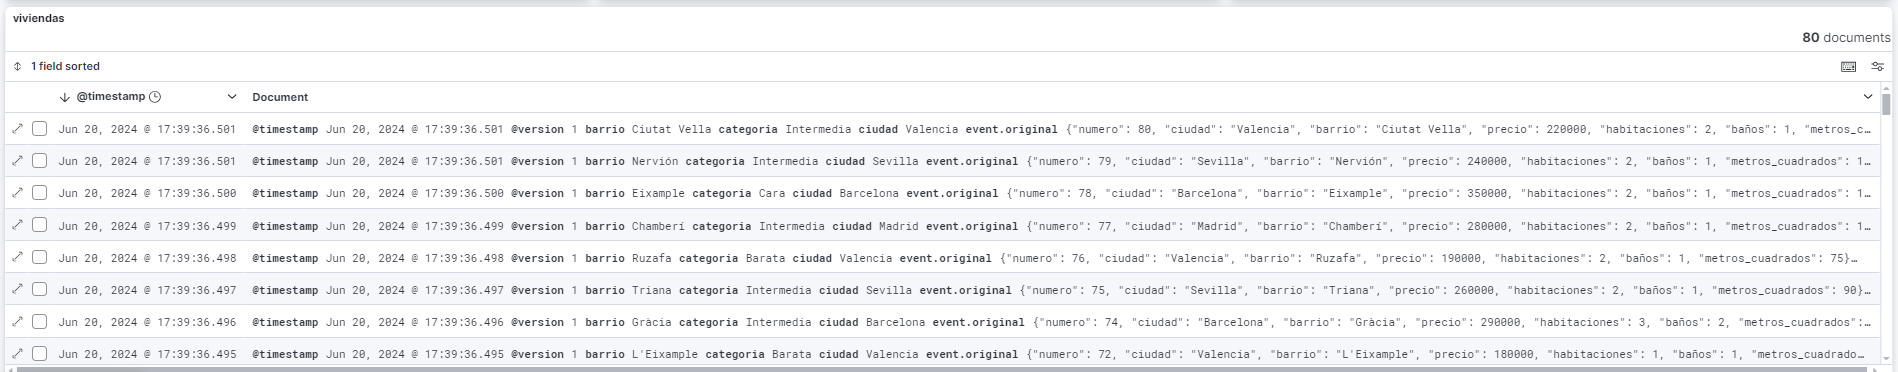
\includegraphics[width=1\linewidth]{img/datosViv.png}
    \caption{Datos del índice del escenario 2}
    \label{fig:datos2}
\end{figure}

\subsubsection{Escenario 3: ingesta a través de WebSocket a Elastic}

El tercer caso se tratará de suscribirse a un data stream a través de la tecnología WebSocket que nos irá mandando datos en tiempo real a Elastic y se irán mostrando en Kibana.

En un principio el tema de los envíos de datos en vivo se planteo como una de las bases del trabajo, puesto que es la situación que más se puede asemejar a un entorno de trabajo con IoT. El problema estaba en que no se disponía de una suscripción a un servicio de ingesta de datos en vivo, por lo que se tuvo que investigar de qué manera se podía implementar esta funcionalidad en el entorno de trabajo. Llegando así al siguiente \href{https://github.com/ColinEberhardt/awesome-public-streaming-datasets}{repositorio} GitHub, el cuál incluía distintos datasets públicos con actualizaciones en vivo.

Tras probar distintos conjuntos de este repositorio, se llegó a la conclusión de que la opción más interesante era la de \href{https://finnhub.io/docs/api/websocket-trades}{Finnhub}, ya que proporciona una \textit{Real-Time RESTful API} y \textit{WebSocket} para interactuar con \textit{stocks} y criptomonedas del mercado.

La \href{https://finnhub.io/}{página oficial} es sencilla de entender, nos proporciona tanto documentación sobre el funcionamiento del \textit{WebSocket}, como una \textit{API key} gratuita para suscribirnos al servicio. Una vez que la tenemos, en la documentación se nos proporciona la estructura básica del script del \textit{WebSocket} escrito en Python. Se debe introducir la \textit{key} obtenida y correr el programa. 

Al ejecutarlo, se mostrara por pantalla las actualizaciones de los distintos precios y características de los símbolos de mercado a los que se haya suscrito en el script. 

En este primer escenario trabajando con \textit{data streams}, la ingesta de datos se hace de la manera más sencilla y estando lo más cerca posible de la fuente de los datos. La información se manda directamente del \textit{WebSocket} a Elastic a través del puerto 9200, llegando al índice "websocket-data", donde los datos en vivo son almacenados, de manera que se pueda usarlos en Kibana para exponerlos y analizarlos en un \textit{dashboard}.

\begin{figure}
    \centering
    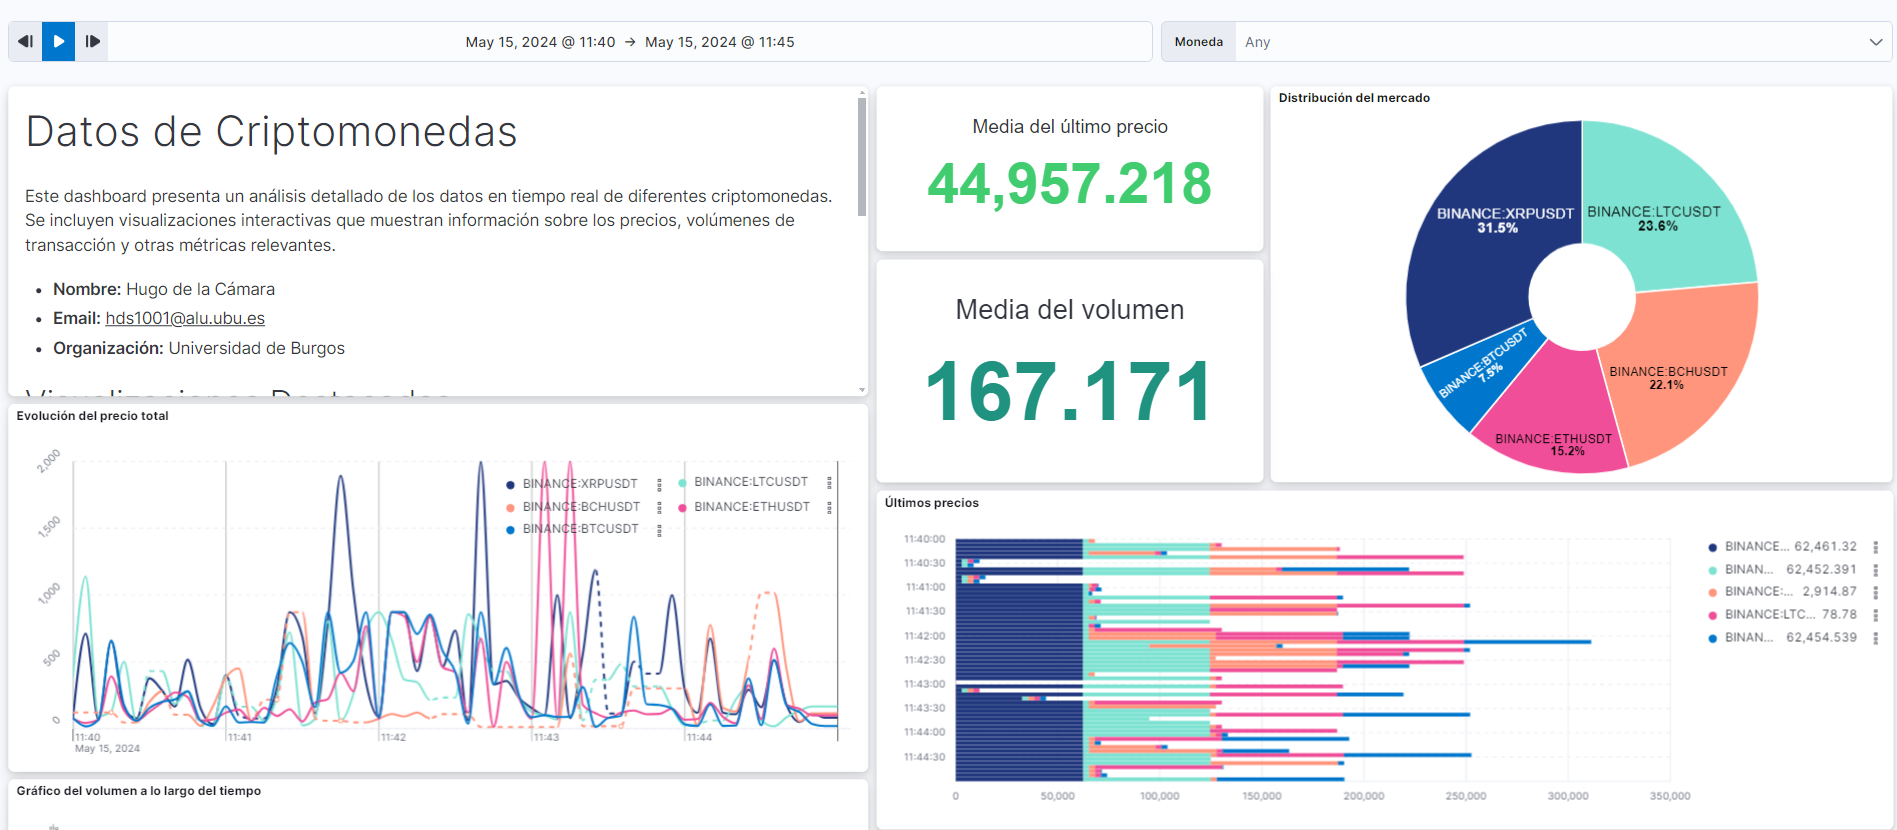
\includegraphics[width=1\linewidth]{img/escenario4-1.png}
    \caption{Dashboard final del tercer escenario}
    \label{fig:escenario3}
\end{figure}
\paragraph{ }
\paragraph{ }
\paragraph{ }
\paragraph{ }
\paragraph{ }
\paragraph{ }
\paragraph{ }
\paragraph{ }
\paragraph{ }
\paragraph{ }
\paragraph{ }
\paragraph{ }
\paragraph{ }
\paragraph{ }
\paragraph{ }

\subsubsection{Escenario 4: ingesta a través de WebSocket con Logstash}

En este cuarto escenario se pretendió rizar el rizo del anterior, y estudiar la posibilidad de modificar esos datos mandados por el WebSocket a través de Logstash antes de mandárselos a Elastic.

Teniendo Logstash presente en el sistema ELK, resulta interesante ver las posbilidades que ofrece a la hora de filtrar y modificar datos en vivo con el apoyo de la documentación presente sobre el tema tanto en la web oficial de Elastic como en foros como StackOverflow.

Para ello, se utilizará el \textit{data stream} del script del tercer escenario, sobre el que se realizarán una serie de modificaciones. La primera va a ser en el mensaje que se manda a Logstash, puesto que las variables sobre cada \textit{stock}, eran mandadas con una letra identificatoria, las cuales sin tener conocimientos sobre el tema, no son comprensibles. Así se modificó la forma en la que se mandaban, cambiando la letra por el nombre completo de la variable en cuestión. 

Tras esto, la siguiente modificación era cambiar el destino de los datos, el cuál ahora iba a ser Logstash. Se utilizó HTTP para realizar este envío en lugar de al puerto 9200 (Elastic) al 8080, en el cuál está Logstash a la escucha de eventos. Con estas modificaciones, al ejecutar el código, los datos son mandados a Logstash para continuar el tratamiento allí.

En Logstash, se aplicaron cambios al mensaje final, eliminando campos vacíos para ahorrar volumen de información, modificando el tipo de las variables para poder realizar posibles operaciones con ellas de manera más sencilla con datos de tipo \textit{float} e \textit{integer}. También se añadieron nuevos campos calculados a partir de los originales calculando el precio total en función del volumen y del último precio de la divisa. Una vez todas las operaciones se han hecho, la información es mandada al puerto 9200 al índice "test-data-stream", para que los datos puedan ser mostrados en un \textit{dashboard} de Kibana. 

\begin{figure}
    \centering
    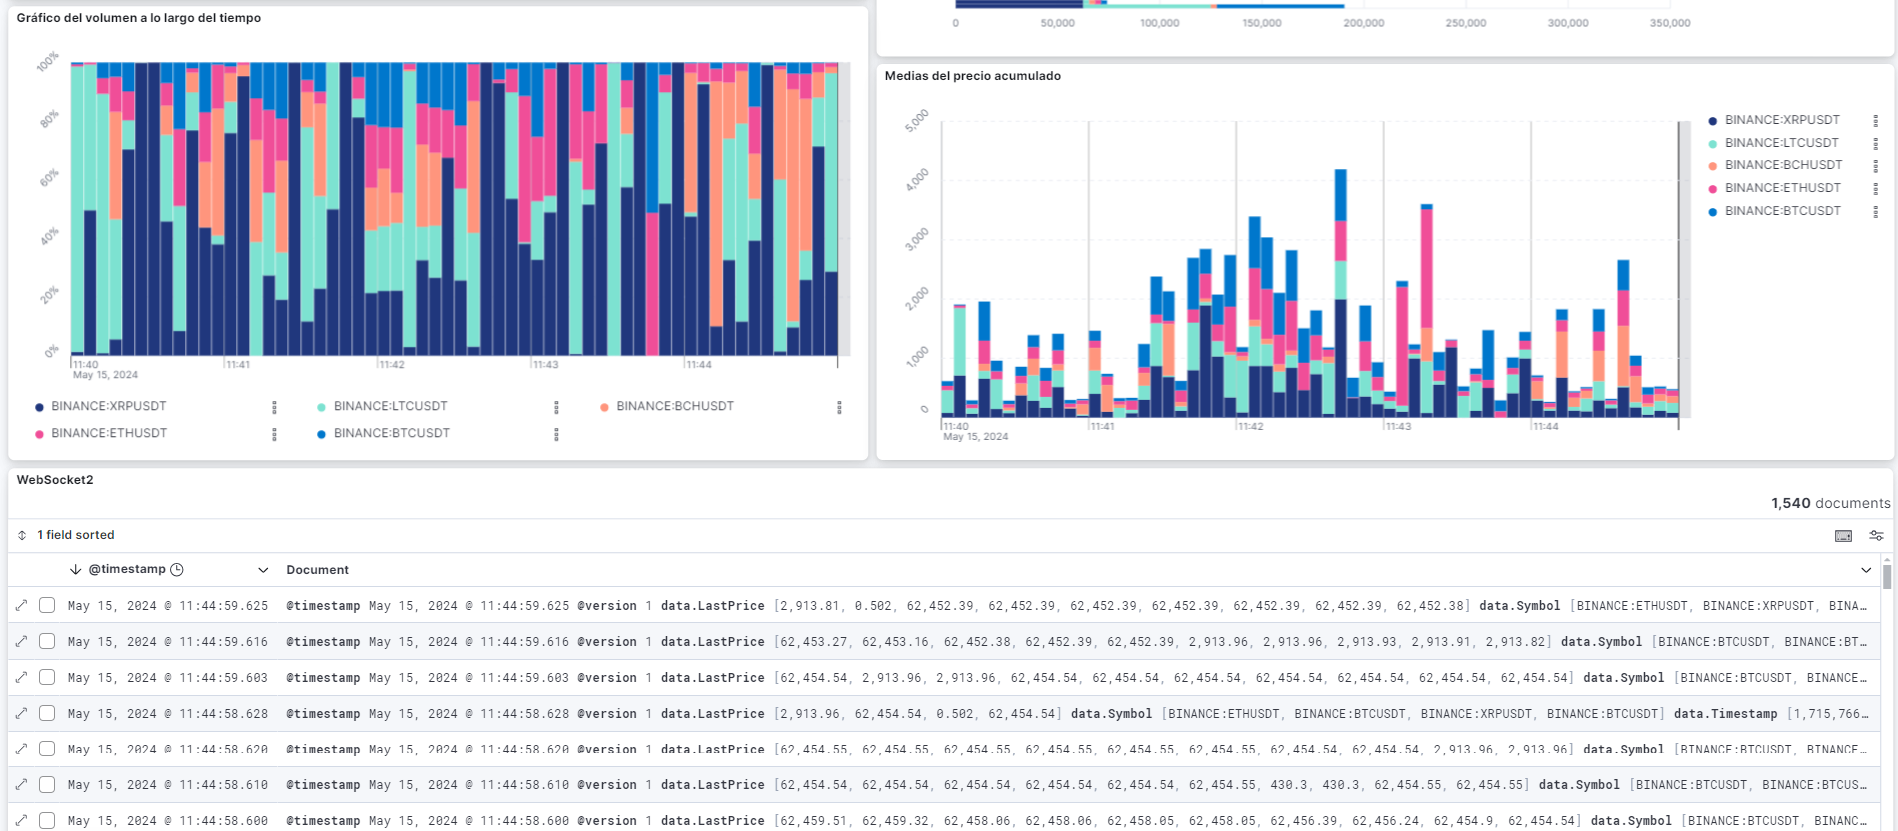
\includegraphics[width=1\linewidth]{img/escenario4-2.png}
    \caption{Dashboard final del cuarto escenario}
    \label{fig:escenario4}
\end{figure}

\paragraph{            }
\paragraph{ }
\paragraph{ }
\paragraph{ }
\paragraph{ }
\paragraph{ }
\paragraph{ }
\paragraph{ }
\paragraph{ }
\paragraph{ }
\paragraph{ }
\paragraph{ }
\paragraph{ }
\paragraph{ }
\paragraph{ }
\paragraph{ }

\subsection{MapReduce para BigData}

En los tiempos que corren, el volumen de transacciones de datos ha aumentado notoriamente, y sigue aumentando a día de hoy. Por lo que los costos de almacenamiento de datos se ha encarecido notablemente. Para reducir estos costes tanto de procesamiento como de almacenamiento, es apropiado utilizar el paradigma de programación  MapReduce, que ya se ha mencionado previamente en los conceptos teóricos. 

Así que una vez se llegó al quinto sprint del proyecto, hubo un enfoque en continuar desarrollando la implementación de MapReduce en una fuente de ingesta de datos sencilla. Por lo que se optó el realizarselo a partir de un fichero de tipo \textit{.log} que contenia distintas transacciones realizadas en una tienda.

\subsubsection{Escenario 5: ingesta de data stream con MapReduce en el servidor mediante Logstash}

En este caso lo que es generar un streaming de datos a partir de un script en Python, cargar esos datos en Logstash, realizarle una serie de modificaciones entre las que se encuentra aplicar el plugin \textit{aggregate}, el cuál cumple el papel de aplicar MapReduce, y cargar esos datos tratados en Elastic para poder visualizarlos en Kibana.

En el data stream sobre el que se va a trabajar, se indican las diferentes transacciones que se han cometido en un comercio con datos sobre las mismas, como el instante de tiempo, el método de pago, la sección en la que se ha comprado, entre otros muchos otros.

Para trabajar con Logstash, se necesita un archivo de configuración para que éste entienda lo que le pedimos que haga. Este archivo es de tipo \textit{.conf} e incluye 3 apartados:
\begin{itemize}
    \item \textbf{Input}: ruta hacia el archivo que contendrá las transacciones
    \item \textbf{Filter}: operaciones a realizarle a estos datos, es decir, el MapReduce con la función \textit{aggregate}
    \item \textbf{Output}: salida por pantalla de los datos mandados a Elastic una vez son tratados.
\end{itemize}

\paragraph{}
\paragraph{}
\paragraph{}


Logstash nos ofrece la función \textit{aggregate}  (ver ilustración  \ref{fig:aggregate}), que permite fusionar muchas líneas de información en una con un determinado criterio en el que se le especifica sobre que campo de los datos va a centrarse. Durante un periodo de tiempo, indicado en la variable \textit{timeout}, la función irá agrupando los registros que concidan con el criterio para que una vez finalizado sean mandados al lugar destino. Se incluirá en el apartado \textit{filter},  indicándole el campo sobre el que hará las agrupaciones en la variable \textit{task id}, así como los datos que se quieren coleccionar una vez son agrupados en la variable \textit{code}. También hay que indicarle un tiempo de inactividad para parar el servicio en la variable \textit{inactivity timeout}.
\begin{figure}
    \centering
    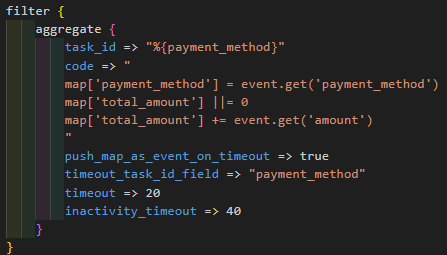
\includegraphics[width=1\linewidth]{img/aggregate.png}
    \caption{Plugin \textit{aggregate} para aplicar MapReduce}
    \label{fig:aggregate}
\end{figure}

En la figura se indica que las agrupaciones se van a realizar en función del método de pago utilizado en cada transacción, y que cada 20 segundos se actualizen estas agrupaciones, y si trás 40 segundos no ha ocurrido ningún cambio, que se detenga el servicio.

En el apartado \textit{output} se indica que los datos procesados seán mandados a ElasticSearch a través del puerto 9200, y que allí se cree un índice con los datos que le lleguen. También se indica que los datos procesados sean mostrados por pantalla para comprobar que todo funciona.

Una vez ejecutado Logstash, a Elastic le llega un índice con tan solo tres filas, las cuáles son las equivalentes a los tres tipos de métodos de pago. Teniendo los datos en el entorno, podemos generar el \textit{dashboard} para mostrarlos y trabajar sobre estas agrupaciones, mostrando el número de compras con cada método de pago en un gráfico de barras horizontal  (ver ilustración  \ref{fig:barras2}), las categorías en las que más se ha gastado  (ver ilustración  \ref{fig:donut2}), los clientes que más han comprado  (ver ilustración  \ref{fig:tabla2}) o el gasto promedio  (ver ilustración  \ref{fig:metrica2}).

\begin{figure}
    \centering
    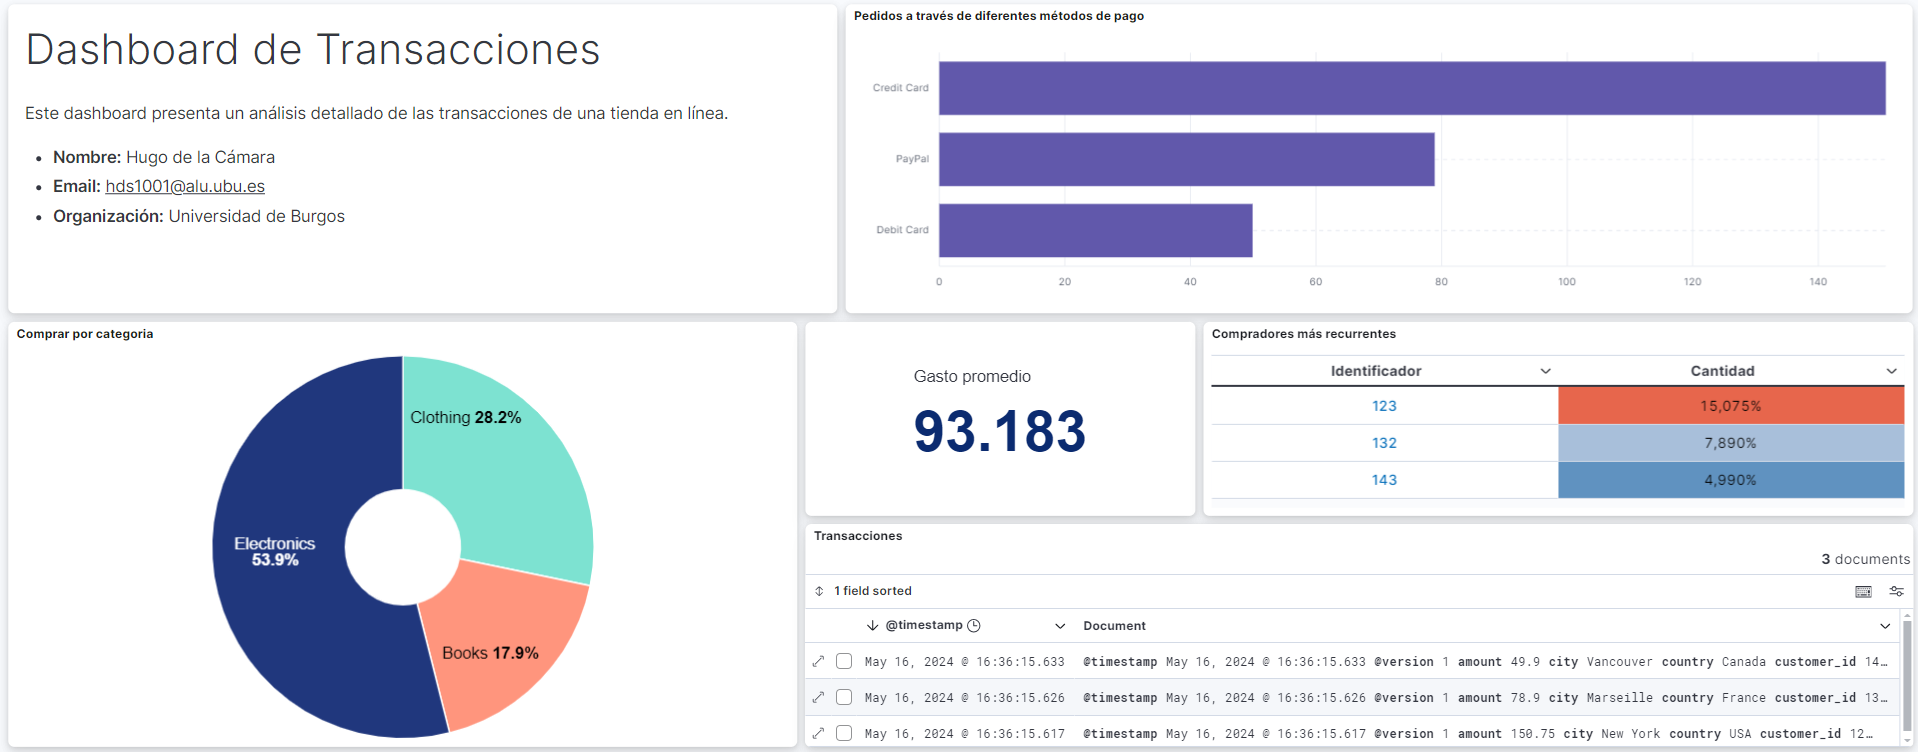
\includegraphics[width=1\linewidth]{img/escenario2.png}
    \caption{Dashboard final del quinto escenario}
    \label{fig:escenario2}
\end{figure}

\begin{figure}
    \centering
    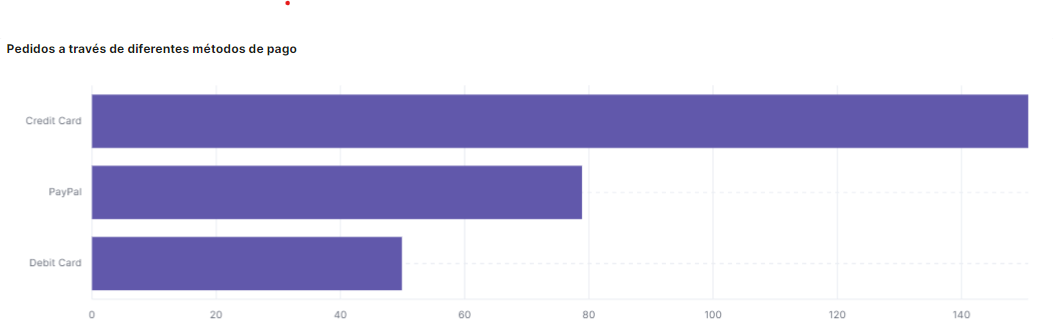
\includegraphics[width=1\linewidth]{img/barras2.png}
    \caption{Gráfico de barras del número de pedidos con cada método de pago}
    \label{fig:barras2}
\end{figure}

\begin{figure}
    \centering
    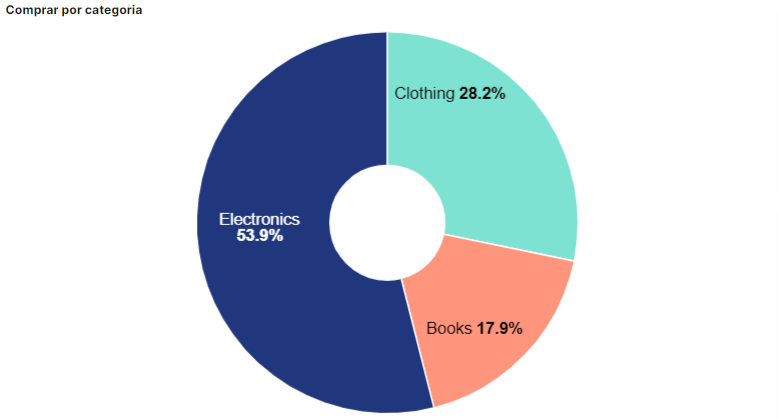
\includegraphics[width=1\linewidth]{img/donut2.png}
    \caption{Gráfico de donut del porcentaje de compra en cada categoría}
    \label{fig:donut2}
\end{figure}

\begin{figure}
    \centering
    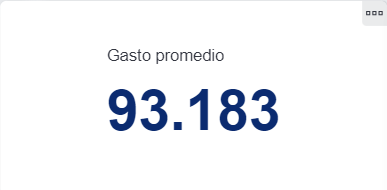
\includegraphics[width=1\linewidth]{img/metrica2.png}
    \caption{Métrica del gasto promedio de cada cliente}
    \label{fig:metrica2}
\end{figure}

\begin{figure}
    \centering
    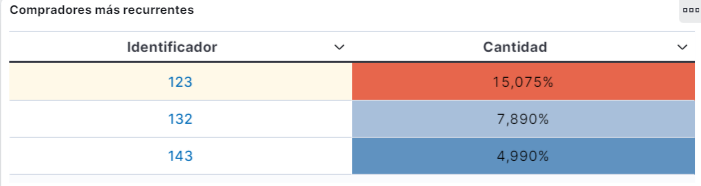
\includegraphics[width=1\linewidth]{img/tabla2.png}
    \caption{Tabla mostrando los clientes más recurrentes}
    \label{fig:tabla2}
\end{figure}


Una vez la carga de los datos en Logstash fue completada con éxito, y se pudo empezar a experimentar con la función que este nos ofrece equivalente a un MapReduce, la función \textit{aggregate}, en la cuál se hizo un agrupado de los datos tomando como referencia el método de pago usado, resultando en que el envío a Elastic fueron 3 lineas con los datos de las cantidades gastadas con cada método y las categorias más compradas entre otros.

\paragraph{}
\paragraph{}

En el caso de este estudio, se aplicó MapReduce a una fuente de datos modesta, puesto que las capacidades de los sistemas en los que se está ejecutando el proyecto son limitadas, pero eso no quita que esta función sea extrapolable a grandes volúmenes de datos con sistemas que sean capaces de procesarlos y reducirlos de cara a moderar el coste de almacenamiento de los mismos. Estos sistemas deben ser clústeres de ordenadores que soporten almacenamiento distribuido , y mediante programas como Hadoop \cite{Hadoop}, esta función se pueda aplicar más fácilmente a grandes masas de datos.

En sistemas de IoT que poseen un gran número de sensores que están mandado datos constantemente es donde resulta interesante aplicar estos conceptos, puesto que se tendrá una estructura ágil para poder analizar la información en tiempo real reduciendo costes.

\paragraph{}
\paragraph{}
\paragraph{}
\paragraph{}
\paragraph{}
\paragraph{}
\paragraph{  }
\paragraph{  }


\subsection{Machine Learning en ELK}

Desde el principio del proyecto se planteó la idea de trabajar con Machine Learning de manera automática con una fuente de ingesta de datos. Al investigar más profundamente, se llegó a la conclusión de que está función si que la ofrece el ecosistema Elastic  (ver ilustración  \ref{fig:machine}), pero pagándola, ya que como se puede observar en la figura las funciones están bloqueadas y solo permite visualizar datos, función que cubre el \textit{Discover}. Hubo que reconducir este escenario de manera que se pudieran aplicar estas técnicas de análisis de manera gratuita.

\begin{figure}
    \centering
    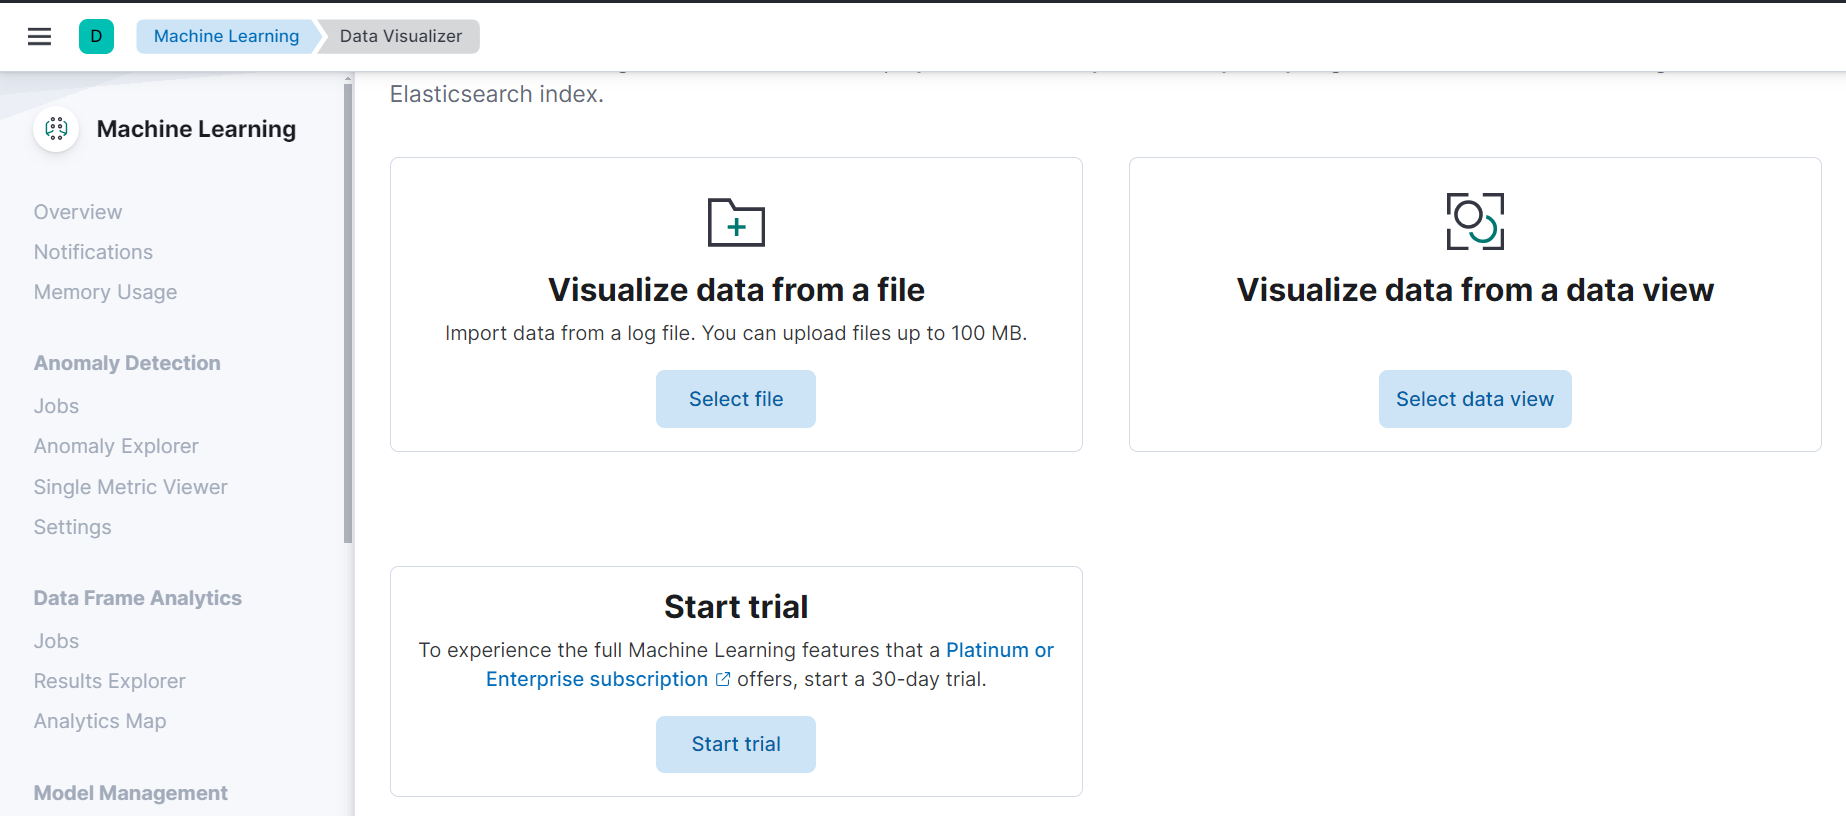
\includegraphics[width=1\linewidth]{img/machineLearning.png}
    \caption{Funcionalidad de Machine Learning de Elastic.}
    \label{fig:machine}
\end{figure}

Y así es como se comenzó a utilizar la biblioteca de análisis predictivo \textit{Scikit-Learn}, la cuál está construida sobre las bibliotecas \textit{Python} de \textit{NumPy}, \textit{SciPy} y \textit{matplotlib}. Para integrar está herramienta en nuestro ecosistema de manera que pudiera interactuar con Elastic, se hizo uso de la herramienta  \textit{Jupyter Notebook}. 

Con \textit{Jupyter}, se generó un script escrito en lenguaje \textit{Python} que importara las librerías necesarias para poder ejecutar los algoritmos de \textit{Scikit-Learn} sobre un conjunto de datos que se le indicara. Como fuente de datos se utilizó un conjunto clásico de las ciencias estadísticas, como lo es el \textit{dataset} Iris, el cuál contiene información sobre tres especies de flores iris, donde cada muestra tiene cuatro características (longitud y anchura del sépalo y del pétalo).

\paragraph{}
\paragraph{}

Lo primero que se hizo fue un script que cargara los datos de Iris en un índice de Elastic, para que un segundo script lea estos desde ese índice, y una vez se tienen los datos cargados en el script desde Elastic, se procede a ejecutar el algoritmo de clasificación \textit{KNN (K vecinos más cercanos)}\cite{knn},  el cuál es un método de clasificación supervisada con el que podemos calcular con qué probabilidad un elemento x desconocido puede pertenecer a una clase a partir de la información que le proporcionemos como prototipo. Una vez se ha obtenido el rendimiento del clasificador, se guardan los resultados localmente en un archivo CSV, y se mandan al puerto 9200 hacia el índice \textit{iris clasificacion}, que será el que almacene los datos en Elastic para que puedan ser mostrados en un \textit{dashboard} de Kibana.

Este proceso de envío de datos va a ser común en los siguientes tres algoritmos que ejecutaremos, siendo el siguiente el de regresión lineal\cite{regresion}, en el cuál se estudia la relación entre la longitud y la anchura de los pétalos de manera que se pueda predecir un comportamiento típico. 

Tras este, vamos a trabajar con algoritmos más visuales, como es el de \textit{clustering} o análisis de grupos con K-Means\cite{clustering} , con el cuál agruparemos los ejemplares de la flor Iris que tengan características similares en diferentes grupos ilustrados con colores. 

Y así concluímos el script con el último algoritmo estudiado, tratándose del de uno reducción de dimensionalidad como es \textit{PCA}\cite{pca}, con el cuál describiremos el conjunto de datos Iris con nuevas variables no correlacionadas, resultando en un gráfico de dispersión bidimensional.

Una vez tenemos toda la información procesada y cargada en Elastic, la creación de un \textit{dashboard} de Kibana viene de la mano, indicándole que los datos se sacarán del índice \textit{Iris} el cuál contiene toda la información que le hemos ido enviando desde el script.

En este \textit{dashboard} se muestran las métricas calculadas por los dos primeros algoritmos  (ver ilustración  \ref{fig:machine1}), y las gráficas calculadas por los dos últimos  (ver ilustraciones  \ref{fig:machine2} y \ref{fig:machine3}, además de información sobre el dataset Iris y los diferentes datos que han cargado los algoritmos como resultado del procesamiento.

\begin{figure}
    \centering
    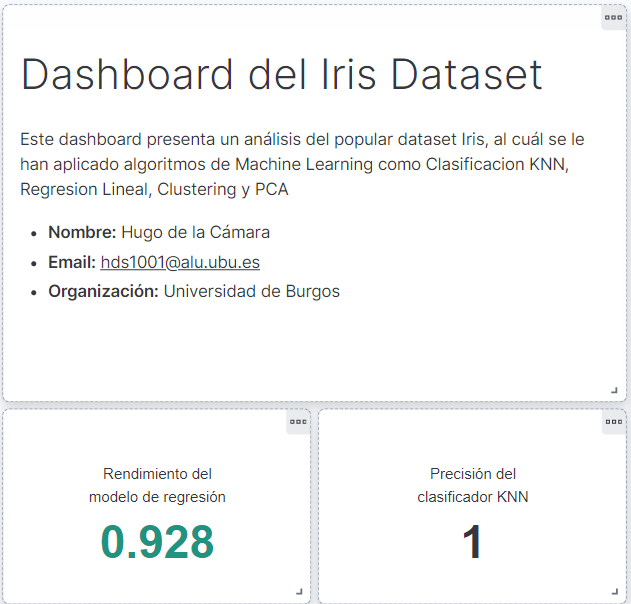
\includegraphics[width=1\linewidth]{img/iris12.png}
    \caption{Visualizaciones mostrando información del \textit{dashboard} así como el rendimiento de la regresión y la precisión del clasificador.}
    \label{fig:machine1}
\end{figure}


\begin{figure}
    \centering
    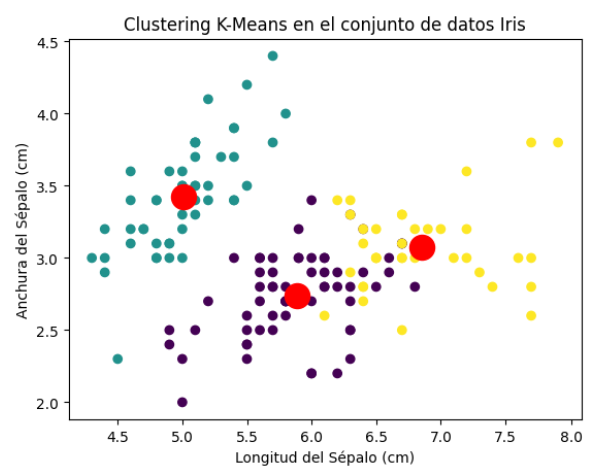
\includegraphics[width=1\linewidth]{img/clustering.png}
    \caption{Visualización de dos dimensiones del gráfico obtenido tras aplicar clustering.}
    \label{fig:machine2}
\end{figure}


\begin{figure}
    \centering
    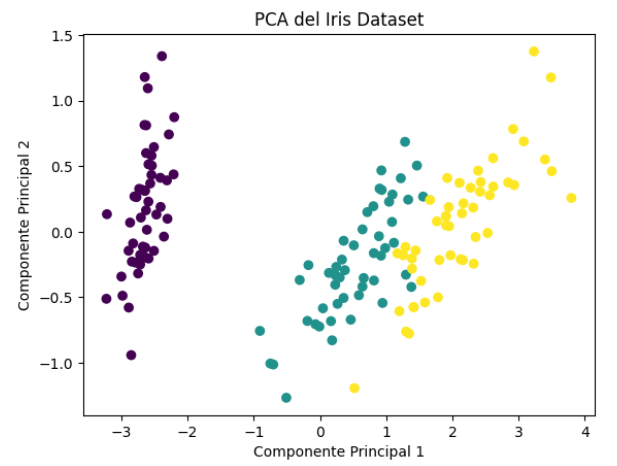
\includegraphics[width=1\linewidth]{img/pca.png}
    \caption{Visualización del gráfico obtenido tras aplicar PCA.}
    \label{fig:machine3}
\end{figure}

\capitulo{6}{Trabajos relacionados}

En este apartado se van a presentar diferentes alternativas de herramientas ETL que cubrán de manera parcial o total los requisitos de las tareas completadas con el sistema ELK.

\section{PowerBI}
Esta herramienta de análisis de datos desarrollada por \textit{Microsoft} está más enfocada al mundo de los negocios\cite{PowerBI}. Y al igual que el \textit{stack ELK} proporciona distintos complementos para realizar visualizaciones de datos y poder crear informes interactivos de los mismos.

A diferencia de el \textit{stack ELK } usado en este proyecto, \textbf{PowerBI} \ref{fig:powerbi}esta basado en la nube, alojando ahi el almacenamiento de los datos, la preparación de estos y las visualizaciones personalizadas.

Por su facilidad de uso, las distintas integraciones que ofrece con programas como \textit{Excel} o \textit{SQL Server}, y sus númerosas funciones avanzadas, \textbf{PowerBI} se destaca como el programa líder del sector y más utilizado a nivel global dento de la ciencia de los datos.

\begin{figure}
    \centering
    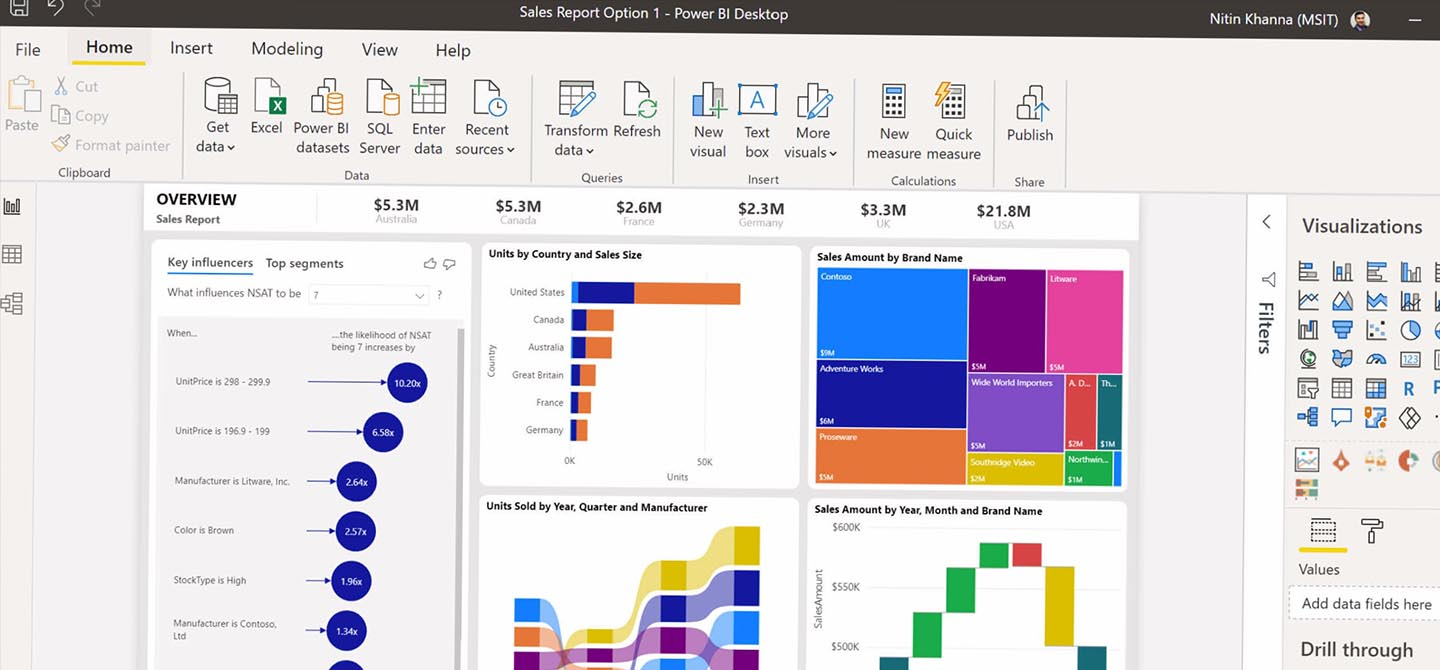
\includegraphics[width=1\linewidth]{img/powerbi.jpg}
    \caption{Visualizaciones de PowerBI \cite{PowerBii}}
    \label{fig:powerbi}
\end{figure}

\paragraph{            }
\paragraph{            }
\paragraph{            }
\paragraph{            }


\section{Spoon y Qlik}
Tuve la oportunidad de realizar las prácticas en la empresa informática CSA (Centro de Servicios Avanzados), concretamente en el departamento de Business Intelligence (BI) y Automatización y Robótica de Procesos (RPA). 

Aquí estuve trabajando con su sistema de herramientas ETL el cuál tenía una estructura diferente pero la finalidad era la misma que la del \textit{Stack ELK}, extraer, transformar y cargar información.

Lo primero era extraer la información de los diferentes servidores y bases de datos de la empresa, y el primer paso para administrar estas bases se hacia a través el programa \textbf{DBeaver}. Una vez teniamos claros los archivos a tratar con la herramienta \textbf{WinSCP} gestionábamos los datos en cuestión. 

La herramienta equivalente a Logstash era \textbf{Spoon} \ref{fig:spoon}, una interfaz para diseñar soluciones de transformación de datos que nos permite crear procesos de carga y lectura de manera intuitiva y visual.

\begin{figure}
    \centering
    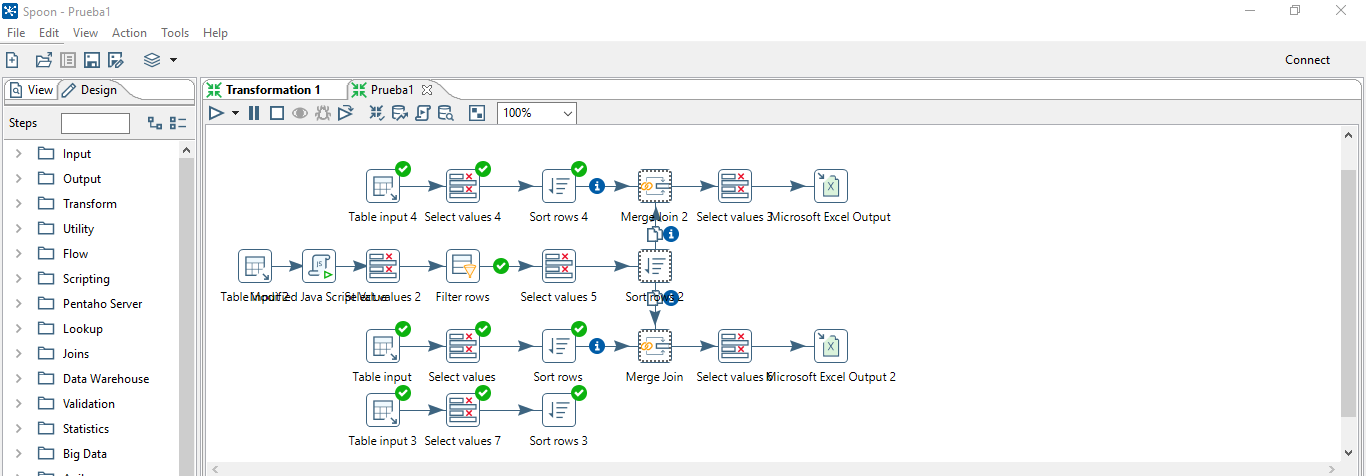
\includegraphics[width=1\linewidth]{img/spoon.png}
    \caption{Estructura de Spoon \cite{Spoon} }
    \label{fig:spoon}
\end{figure}

Y por último, la herramienta estrella, \textbf{Qlik}  \ref{fig:qlik}, que nos permite pintar gráficos e interfaces con todos los datos procesados por las herramientas anteriores.

\begin{figure}
    \centering
    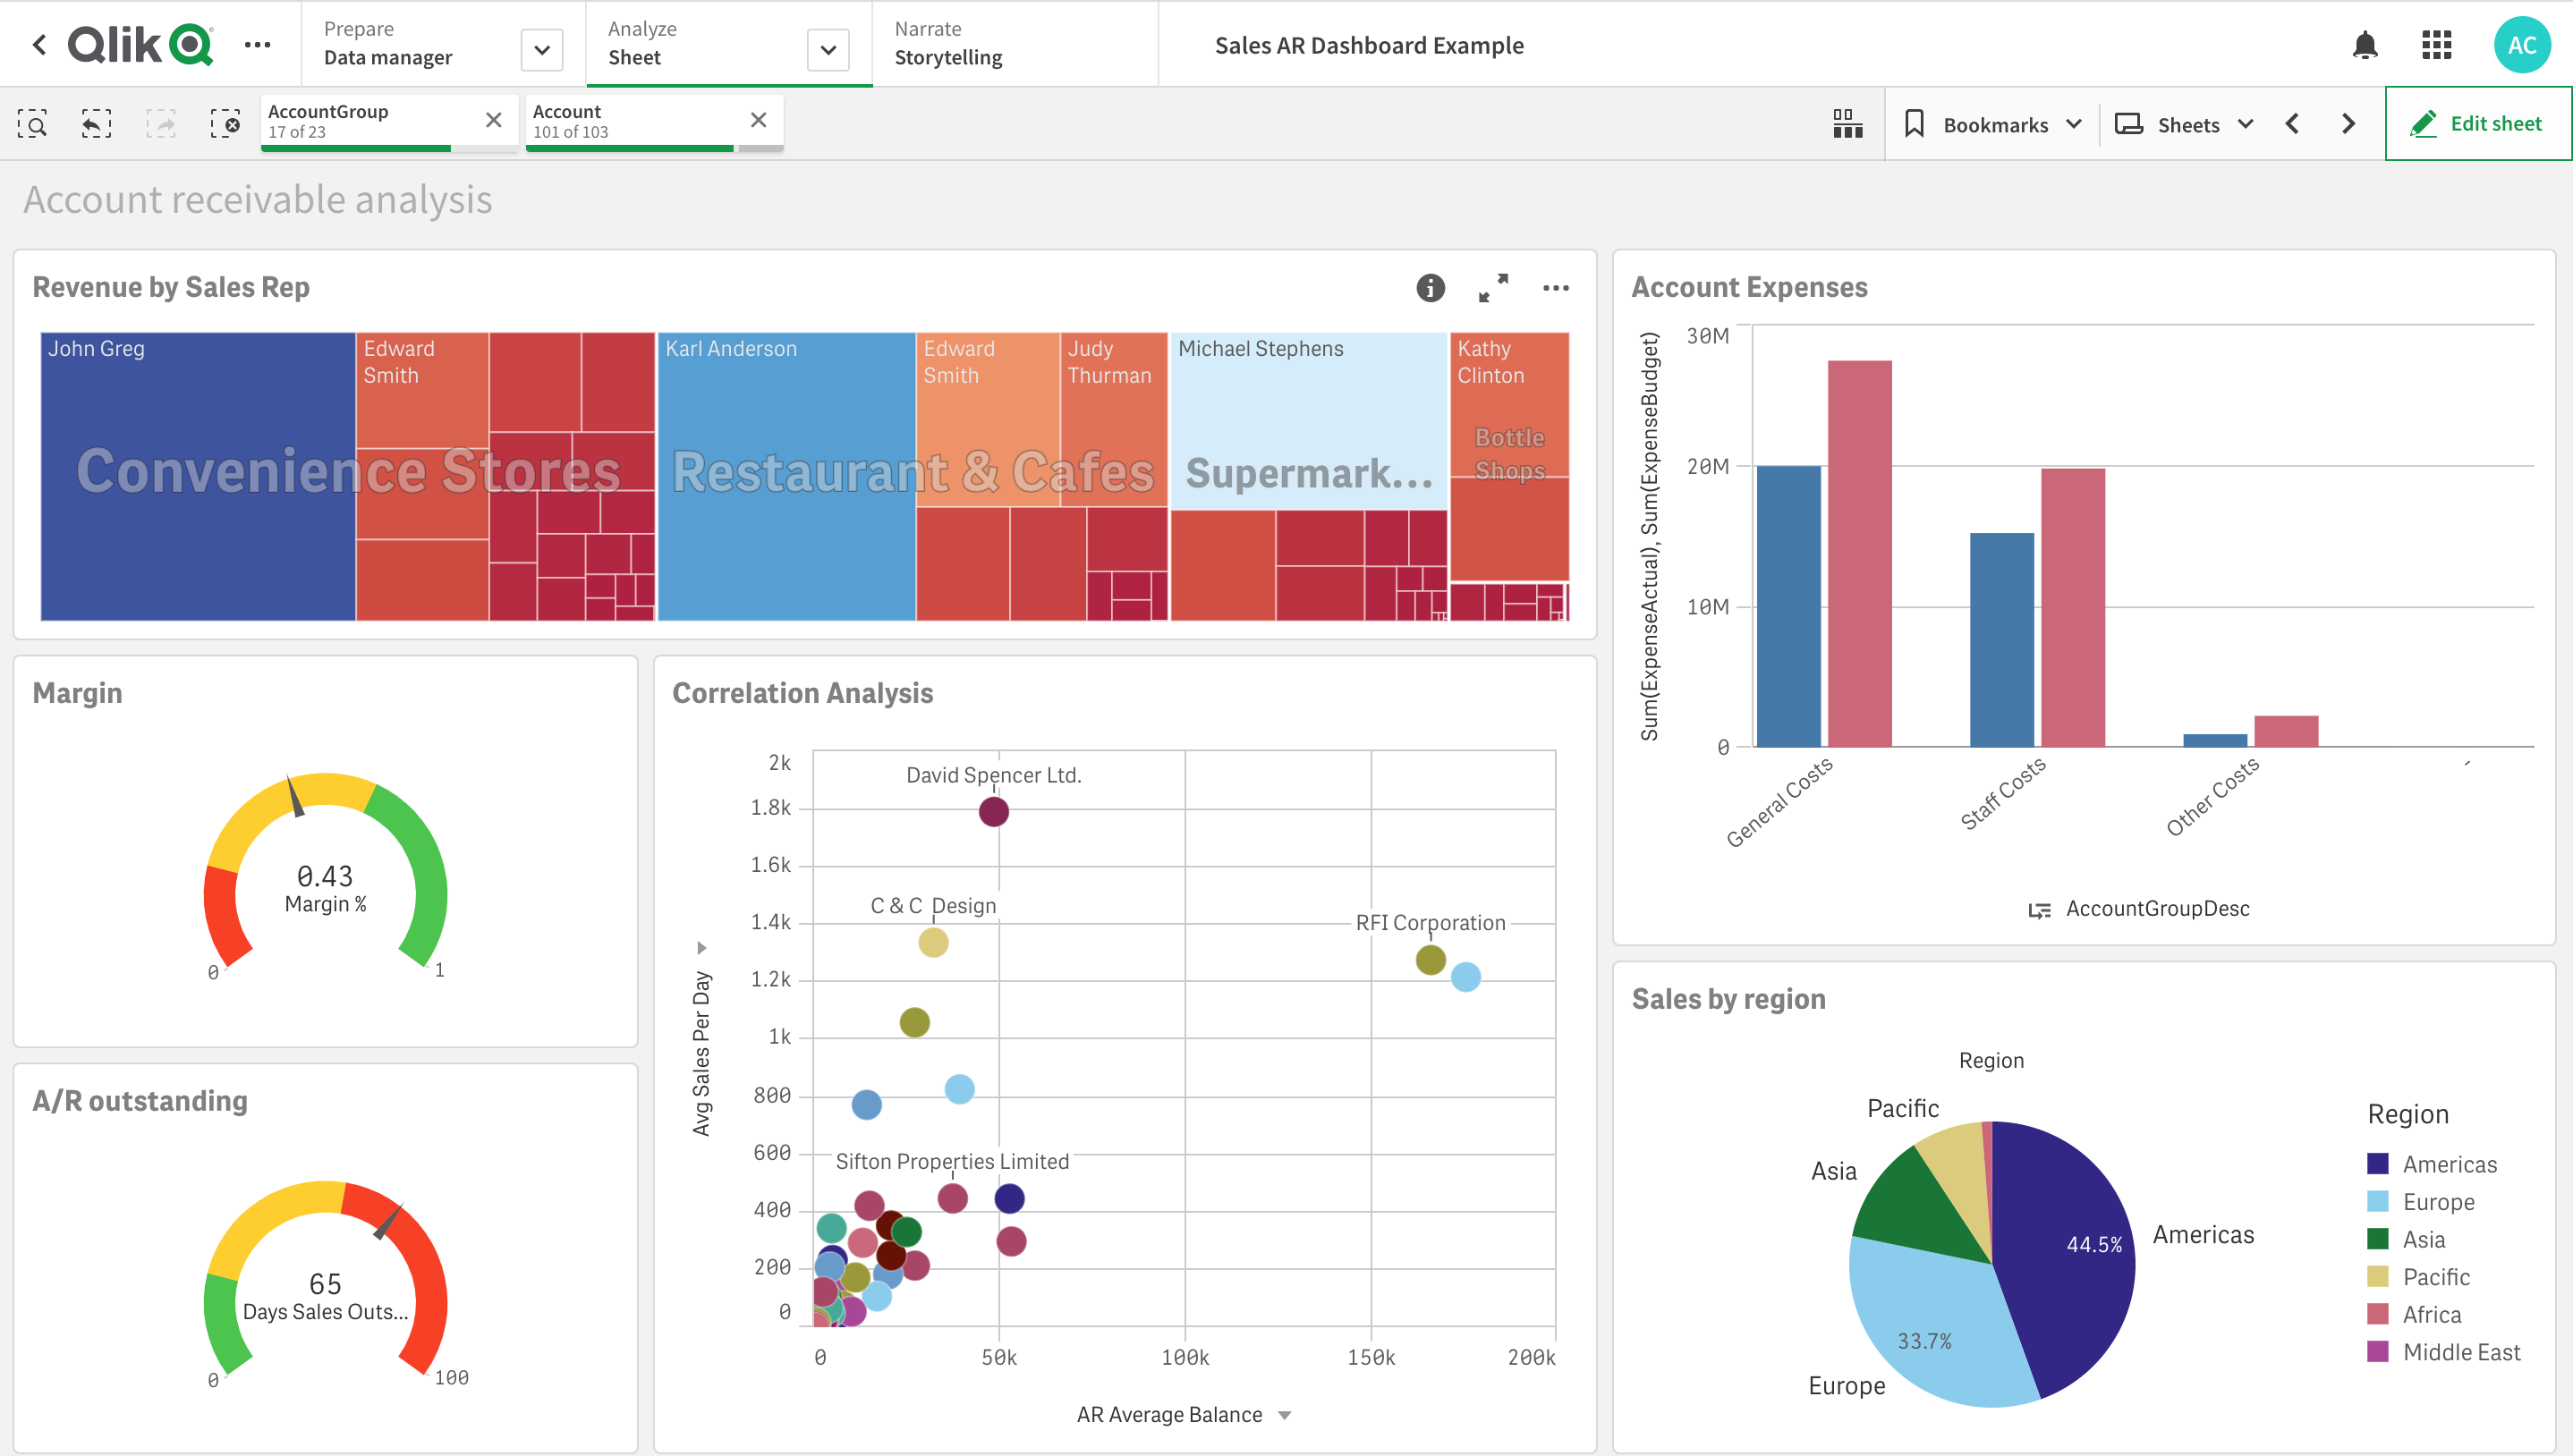
\includegraphics[width=1\linewidth]{img/qlik.png}
    \caption{Visualizciones con Qlik \cite{Qlik} }
    \label{fig:qlik}
\end{figure}

\paragraph{            }
\paragraph{            }

\section{Tableau}
Este software está pensado para el desarrollo de visualizaciones interactivas  de datos en forma de gráficos en \textit{dashboards} \ref{fig:tableau}. Fue diseñado para el análisis y comprensión de datos complejos ya que soporta la ingesta de datos tanto desde hojas de cálculo como de bases de datos. Posee una interfaz intuitiva basada en \textit{drag and drop} de manera que cualquier usuario pueda comprender y tomar decisiones basadas en información de datos.

\begin{figure}
    \centering
    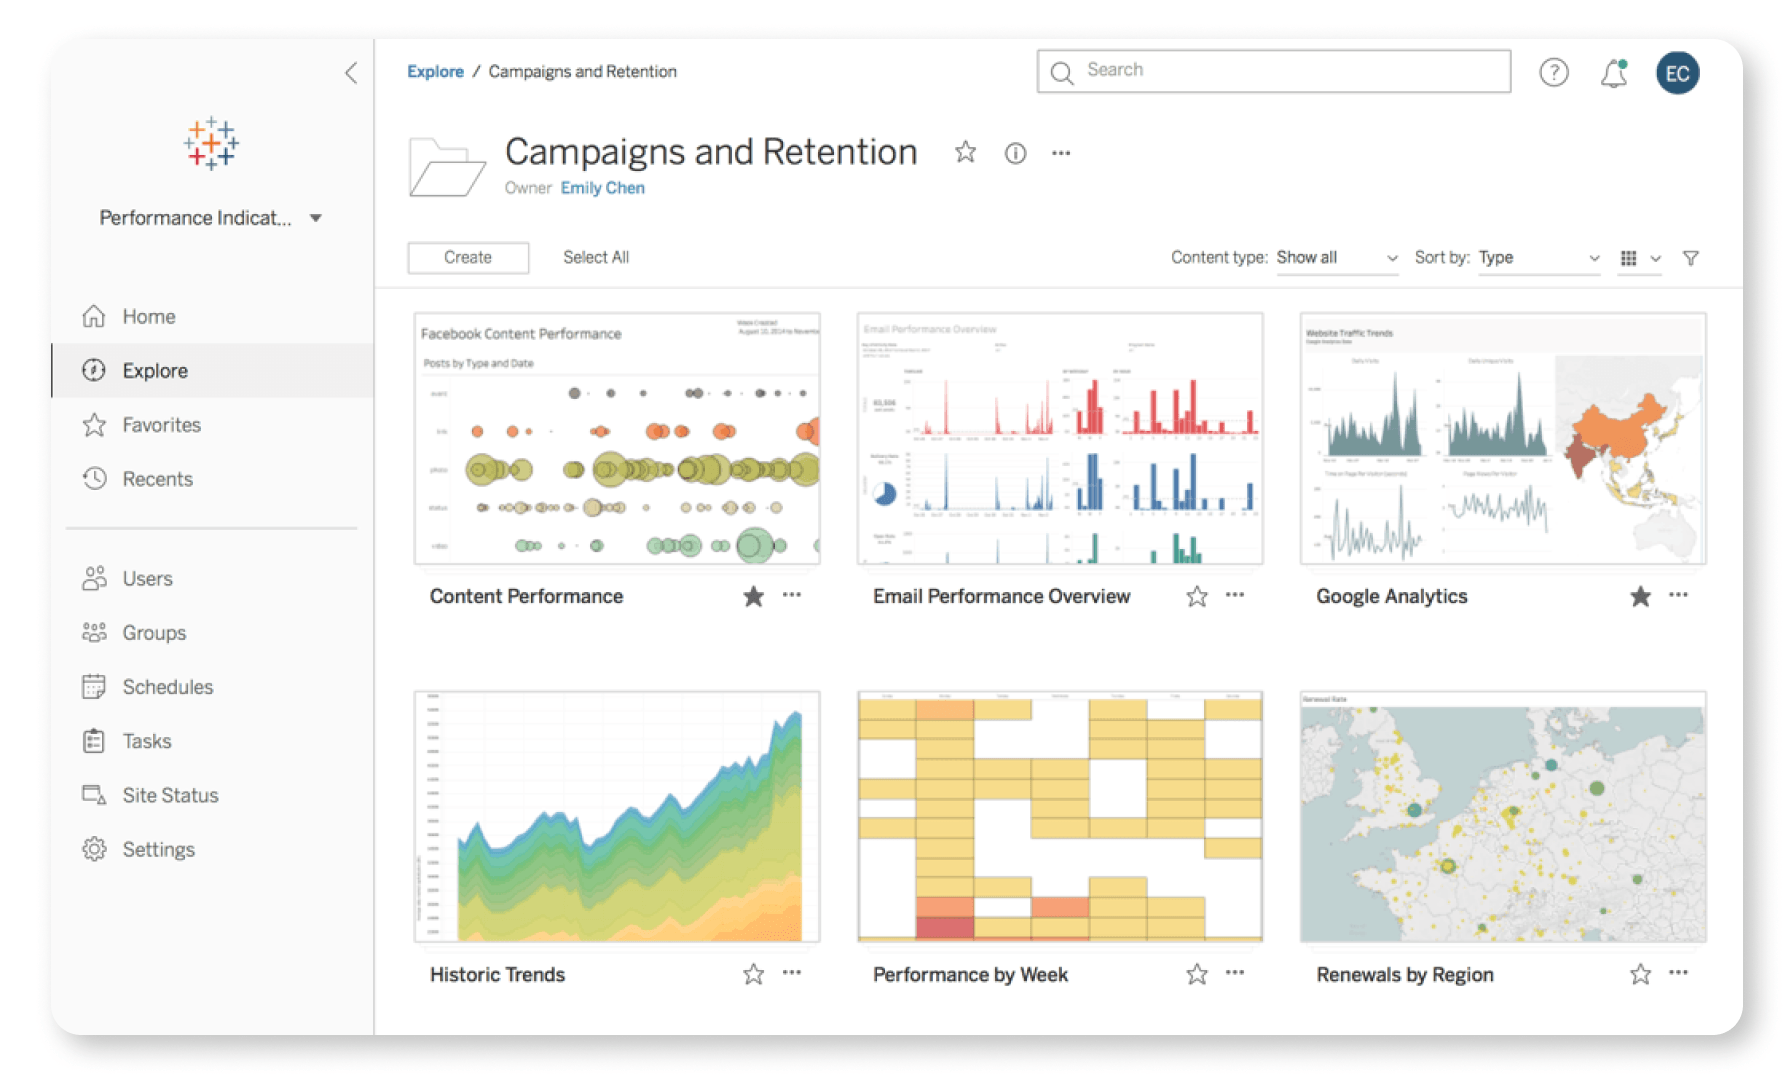
\includegraphics[width=1\linewidth]{img/tableau.png}
    \caption{Dashboard principal de Tableau \cite{tableau}}
    \label{fig:tableau}
\end{figure}
\section{Splunk}
Consiste en una plataforma diseña para analizar y monitorear datos ingestados en tiempo real \ref{fig:splunk}. Este software recopila e indexa grandes conjuntos de datos de manera que se puedan filtrar y analizar de manera profunda y avanzada a la hora de identificar anomalías, optimizar procesos o identificar patrones.

\begin{figure}
    \centering
    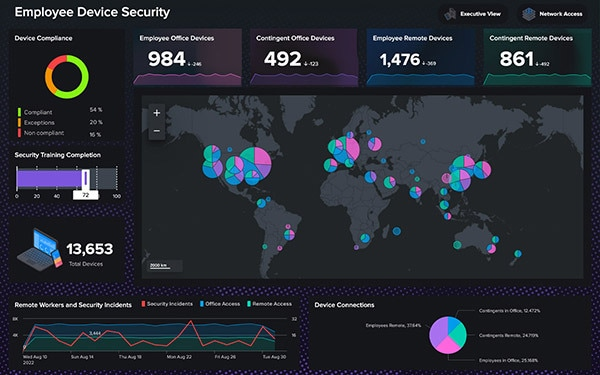
\includegraphics[width=1\linewidth]{img/splunk.jpg}
    \caption{Dashboard básico de Splunk \cite{splunk}}
    \label{fig:splunk}
\end{figure}

\section{Comparativa entre alternativas}

A continuación se realizará una tabla comparativa entre las diferentes opciones expuestas en este apartado como alternativas al stack ELK, así como más opciones presentes en el mercado. Se incluyen algunas características o propiedas que resultan interesantes. \ref{tab:comparacion}

Cabe destacar que las funciones de inteligencia artificial en el caso del stack ELK se considerena limitadas, ya que ofrece detección de anomalías y un plugin para uso de machine learning. Ambas funciones solo están disponibles en el plan de suscripción Platinum, por lo que se consideran escasas en comparación con PowerBI, el cuál integra machine learning para realizar modelos predictivos o analizar series temporales. Qlik, Tableau y Splunk ofrecen características muy similares de este tipo sobre todo enfocadas al análisis y procesamiento de datos en tiempo real.

Como conclusión indicar que el stack ELK está pensado para monitorizar y analizar datos, principalmente de tipo log, en tiempo real, no como PowerBi que está más enfocado al ámbito empresarial a la hora de generar informes (ideal si el ecosistema en el que se trabaja es el de Microsoft). Qlik y Spoon son una buena combinación para negocios basados en ETL, al igual que Tableau y Splunk al ser todas herramientas para usos muy similares.


\begin{table}[h]
\centering
\begin{tabularx}{\textwidth}{|X|X|X|X|X|X|}
\hline
 & \textbf{Stack ELK} & \textbf{Power BI} & \textbf{Qlik + Spoon} & \textbf{Tableau} & \textbf{Splunk} \\ \hline
\textbf{Función principal} & Análisis de logs y datos en tiempo real & Análisis de negocios y generación de informes & Análisis de negocios y ETL & Visualización de datos de negocios & Análisis de datos en tiempo real \\ \hline
\textbf{Facilidad de uso} & Requiere conocimientos técnicos avanzados & Interfaz intuitiva y fácil de usar & Qlik es más intuitivo que Spoon & Interfaz intuitiva y fácil de usar & Requiere conocimientos técnicos avanzados \\ \hline
\textbf{Escalabilidad} & Alta & Limitada & Alta & Alta & Alta \\ \hline
\textbf{Coste} & Gratis, opciones avanzadas de pago & Suscripción de pago & Qlik licencia de pago, Spoon es gratis & Suscripción de pago & Suscripción de pago \\ \hline
\textbf{Almacenamiento en la Nube} & Lo proporciona el servicio de pago Elasticsearch Service & Sí, integrado con Azure & Qlik sí que lo ofrece y Spoon puede integrarse & Sí, integrado con servicios en la nube & Sí, integrado con servicios en la nube \\ \hline
\textbf{Análisis en Tiempo Real} & Sí, nativo & Depende de la fuente de datos & Sí, Qlik permite análisis en tiempo real & Depende de la fuente de datos & Sí, nativo \\ \hline
\textbf{Inteligencia Artificial} & Funcionalidades limitadas & Ofrece capacidades de IA y análisis predictivo & Qlik tiene capacidades de IA, Spoon no & Ofrece IA y análisis predictivo & Ofrece IA y análisis predictivo \\ \hline
\textbf{Sistemas Operativos} & Windows, Linux y Mac & Windows y Mac & Windows, Linux y Mac & Windows, Linux y Mac & Windows, Linux y Mac \\
\end{tabularx}
\caption{Comparación entre herramientas ETL}
\label{tab:comparacion}
\end{table}

\capitulo{7}{Conclusiones y Líneas de trabajo futuras}

El último apartado de este documento memoria va a consistir en la redacción de las conclusiones y valoraciones finales del proyecto, así como diferentes mejoras que se le podrían realizar de cara a un futuro.

\section{Conclusiones}

A lo largo de este estudio se han planteado objetivos que se han podido conseguir y que se van a remarcar en este apartado de que manera se que han conseguido, y otros que no han sido posibles y que se dejan como posibles mejoras en el siguiente apartado de cara a trabajos futuros.

Se ha logrado crear cinco escenarios que muestran diferentes maneras ingestar datos con el stack ELK, ya sea a través de un fichero estático o un data stream, aplicándole modificaciones de cara al producto final mostrado.

No se ha podido realizar escenarios con otras fuentes de datos puesto que suponía aumentar la carga de trabajo. Se intentó crear un escenario en el que se mandarán datos desde \textit{Filebeat}, pero no se pudo lograr por la dificultad de comprensión del mismo. Por lo que como sustituto se recurrió a los WebSockets para que cubrieran la función de ingesta de data streeams en el tercer y cuarto escenario. 

\paragraph{}
\paragraph{}
\paragraph{}

No obstante, desde el punto de vista funcional, los resultados se consideran extrapolables a conjuntos de datos de gran tamaño. Sin embargo, ha quedado por explorar cómo optimizar la configuración de un sistema hardware de gran potencia, típicamente un cluster, para optimizar el rendimiento del \textit{stack ELK} ante situaciones de ingesta masiva. Este punto se ha quedado fuera del alcance del TFG por falta de recursos hardware. 

En general la experiencia ha resultado enriquecedora e interesante por el hecho de poder aplicar conocimientos que se han adquirido estos últimos años y que han resultado útiles en el desarrollo del proyecto. La documentación presente sobre las herramientas era escasa en ciertos ámbitos por lo que este aspecto a dificultado parte del estudio.

\section{Mejoras futuras}
De cara a continuar con este trabajo se considera que se le podrían aplicar ciertos matices para que los escenarios puedan ser más completos y útiles.
\begin{itemize}
    \item Realizar pruebas de tiempos de respuesta para calcular la eficiencia del \textit{stack ELK} en comparación a otros programas como PowerBI.
    \item Incluir más escenarios utilizando como origen de los datos \textit{Filebeat} o algún otro API diferente.
    \item Mejorar la calidad de los datos, incluyendo que su limpieza y normalización se realice mas eficientemente.
\item Explorar nuevos escenarios que combinen datos de múltiples orígenes.
\item Probar la arquitectura ELK sobre un sistema de Big Data con Hadoop.
\item Intentar programar y publicar un plugin para Elasticsearch orientado a incorporar técnicas de Machine Learning. 
\end{itemize}


\bibliographystyle{plain}
\bibliography{bibliografia}



\end{document}
